\documentclass[dvipdfmx]{jsarticle}
\usepackage{penrosetensor}

\begin{document}

\section{行列と行列式の表現}
\label{sec: matrix}

\subsection{前提知識}

本節では,
\begin{itemize}
    \item 学部教養課程の線形代数
    \item Einsteinの縮約記法
    \item 完全反対称Levi-Civita記号とグラフ記法による表記
    \item Kroneckerの$\delta$とグラフ記法による表記
\end{itemize}
についての知識を前提とする.


\subsection{Penroseのグラフ記法を用いた行列の表記}
\label{sec: matrix: display of matrix}

本節での記法は正方行列であればある程度非正則でも使用できる.
また一部の記述について, 正方行列に限らない任意の行列に拡張可能である.

以降, 行列のうち行の添字を上付き, 列の添字を下付きで表すことにする.
例えば
\begin{align*}
    M=\mqty(a&b\\c&d)\Longrightarrow M^1_2=b
\end{align*}
である.
列ベクトルの成分を$u^i$, 行ベクトルの成分を$v_j$で表すことにする.
\begin{equation*}
    \bm{u}
    =
    \mqty(a\\b)
    \Longrightarrow
    u^1=a,
    \qquad
    \bm{v}
    =
    \mqty(a&b)
    \Longrightarrow
    v_2=b.
\end{equation*}
正方行列を扱う場合, $n$は行列の次元$n=\dim A$とする.



\subsubsection{行列・ベクトル}

グラフ記法で行列$A$は上下または左右から脚が生えたものとして表される.
\begin{equation*}
    A=
    \vcenter{\hbox{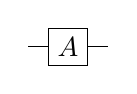
\begin{tikzpicture}
    \node at(0,0)[anchor=center, draw, rectangle](A){$A$};
    \draw
        (A.east)--++(.25,0)
        (A.west)--++(-.25,0)
    ;
\end{tikzpicture}
}}
\end{equation*}
本節では右左の脚をそれぞれ行, 列の添字に対応させる.
これに従い$A^i_j$は
\begin{equation*}
    A^i_j
    =
    \vcenter{\hbox{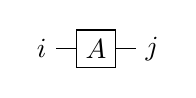
\begin{tikzpicture}
    \node at(0,0)[anchor=center, draw, rectangle](A){$A$};
    \draw
        (A.west)--++(-.25,0)node[left]{$i$}
        (A.east)--++(.25,0)node[right]{$j$}
    ;
\end{tikzpicture}
}}
\end{equation*}
と書ける.

1階のテンソルであるベクトルは\ref{sec: vector}同様に脚が1本生えたものとして表すが, 列ベクトルと行ベクトルの区別が必要となる.
本節では脚が右に生えたら行ベクトル, 左に生えたら列ベクトルと約束する.
\begin{equation*}
    u_i=
    \vcenter{\hbox{\documentclass[dvipdfmx]{jsarticle}
\usepackage{penrosetensor}

\begin{document}

\section{ベクトル解析の公式の表現}
\label{sec: vector}

\subsection{前提知識}

本節では
\begin{itemize}
    \item スカラーとベクトルの区別
    \item ベクトルの内積と外積の定義
    \item grad, div, rot, $\lapl$
    \item Einsteinの縮約記法
    \item Kroneckerの$\delta$
    \item Levi-Civita記号とその縮約公式
    \item 外積のLevi-Civita記号による表示
\end{itemize}
の知識を前提とする.

基本的に添字を使う場合はEinsteinの縮約記法に従って表す.
また, 本節では共変・反変の区別をせず, Einsteinの縮約記法の添字は全て下付きとする.


\subsection{スカラーとベクトルおよび演算の定義}

\subsubsection{スカラーとベクトルの表示}

グラフ記法においてスカラーは文字を四角く囲って表される.
\begin{equation*}
    \text{scalar}\:f=\vcenter{\hbox{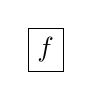
\begin{tikzpicture}
    \node at(0,0)[anchor=north, draw, rectangle]{$f$};
\end{tikzpicture}
}}
\end{equation*}
ベクトルは脚つきで表現される.
\begin{equation*}
    \text{vector}\:\bm{v}=\vcenter{\hbox{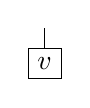
\begin{tikzpicture}
    \node at(0,0)[anchor=north, draw, rectangle](v){$\bm{v}$};
    \draw(v.north)--++(0,.25);
\end{tikzpicture}
}}
\end{equation*}
この脚は\ref{sec: Kronecker for tensor}に示すようにKroneckerの$\delta$を表す.


\subsubsection{スカラー倍}

文字式と同様, スカラーとベクトルを並べてスカラー倍を表せる.
\begin{equation*}
    fg\bm{v}
    =
    \vcenter{\hbox{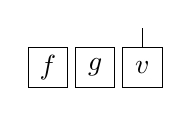
\begin{tikzpicture}
    \draw(-.6,0)rectangle(-.1,.5);
    \draw(0,0)rectangle(.5,.5);
    \draw(.6,0)rectangle(1.1,.5);
    \draw(.85,.5)--(.85,.75);
    \node[anchor=center]at(-.35,.25){$f$};
    \node[anchor=center]at(.25,.25){$g$};
    \node[anchor=center]at(.85,.25){$\bm{v}$};
\end{tikzpicture}
}}
\end{equation*}


\subsubsection{ベクトルの内積}

ベクトルの脚を繋ぎ合わせると内積を表す.
\begin{equation*}
    \bm{u\cdot v}=u_i\delta_{ij}v_j
    =
    \vcenter{\hbox{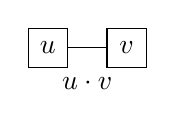
\begin{tikzpicture}
    \draw(0,0)rectangle(.5,.5);
    \draw(1.,0)rectangle(1.5,.5);
    \draw(.5,.25)--(1.,.25);
    \node[anchor=center]at(.25,.25){$\bm{u}$};
    \node[anchor=center]at(1.25,.25){$\bm{v}$};
    \node[anchor=north]at(.75,0){$\bm{u\cdot v}$};
\end{tikzpicture}
}}
\end{equation*}


\subsubsection{3成分のLevi-Civita記号}
\label{sec: vector: 3 components levicivita}

以上ではスカラーやベクトルは四角で囲って表してきたが, ベクトルの添字については四角で囲わずに表すこととする.
この約束のもと, 3成分のLevi-Civita記号は次のように表す.
\begin{equation*}
    \epsilon_{ijk}
    =
    \vcenter{\hbox{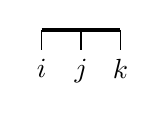
\begin{tikzpicture}
    \draw[ultra thick]
        (0,1)--(1,1)
    ;
    \draw
        (0,1)--(0,.75) node[anchor=north]{$i$}
        (.5,1)--(.5,.75) node[anchor=north]{$j$}
        (1,1)--(1,.75) node[anchor=north]{$k$}
    ;
\end{tikzpicture}
}}
\end{equation*}
太線は反対称性を表し, 脚の奇置換で符号が変わる.
\begin{equation*}
    \vcenter{\hbox{\input{img/vector/levicivita-ikj.tex}}}
    =
    -\vcenter{\hbox{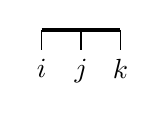
\begin{tikzpicture}
    \draw[ultra thick]
        (0,1)--(1,1)
    ;
    \draw
        (0,1)--(0,.75) node[anchor=north]{$i$}
        (.5,1)--(.5,.75) node[anchor=north]{$j$}
        (1,1)--(1,.75) node[anchor=north]{$k$}
    ;
\end{tikzpicture}
}}
\end{equation*}


\subsubsection{ベクトルの外積}

ベクトルの外積は次のように表せる.
\begin{equation*}
    \bm{u}\times\bm{v}
    =
    \vcenter{\hbox{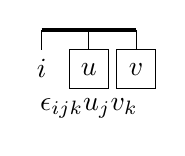
\begin{tikzpicture}
    \draw[ultra thick]
        (.25,1)--(1.45,1)
    ;
    \draw
    (.25,1)--(.25,.75) node[anchor=north]{$i$}
    (.85,1)--(.85,.75)
    (1.45,1)--(1.45,.75)
    (.6,.25)rectangle(1.1,.75)
    node[anchor=center]at(.85,.5){$\bm{u}$}
    (1.2,.25)rectangle(1.7,.75)
    node[anchor=center]at(1.45,.5){$\bm{v}$}
    ;
    \node[anchor=north]at(.85,.25){$\epsilon_{ijk}u_jv_k$};
\end{tikzpicture}
}}
\end{equation*}
一番左に脚が1本残っていることからベクトルであることが一瞥できる.



\subsection{ベクトルの内積と外積にまつわる公式}

\subsubsection{Levi-Civita記号の縮約公式}
\label{sec: levi-civita contraction for vectors}

\begin{equation*}
    \epsilon_{ijm}\epsilon_{klm}
    =
    \delta_{ik}\delta_{jl}
    -
    \delta_{il}\delta_{jk}
\end{equation*}
Levi-Civita記号の縮約公式は\ref{sec: levicivita: contraction}で詳細を取り扱うが, ここでは公式的に用いることにする.
\begin{equation*}
    \vcenter{\hbox{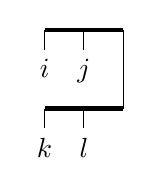
\begin{tikzpicture}
    \draw[ultra thick]
        (0,1)--(1,1)
        (0,2)--(1,2)
    ;
    \draw
        (0,1)--(0,.75) node[anchor=north]{$k$}
        (.5,1)--(.5,.75) node[anchor=north]{$l$}
        (1,1)--(1,2)
        (0,2)--(0,1.75) node[anchor=north]{$i$}
        (.5,2)--(.5,1.75) node[anchor=north]{$j$}
    ;
\end{tikzpicture}
}}
    =
    \vcenter{\hbox{\begin{tikzpicture}
    \draw
        node (i1) at (2,1.25) [anchor=south]{$i$}
        node (j1) at (2.5,1.25)[anchor=south]{$j$}
        node (k1) at (2,.75) [anchor=north]{$k$}
        node (l1) at (2.5,.75) [anchor=north]{$l$}
        (i1) -- (k1)
        (j1) -- (l1)
    ;
\end{tikzpicture}
}}
    -
    \vcenter{\hbox{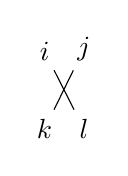
\begin{tikzpicture}
    \draw
        node (i2) at (3.5,1.25) [anchor=south]{$i$}
        node (j2) at (4,1.25)[anchor=south]{$j$}
        node (k2) at (3.5,.75) [anchor=north]{$k$}
        node (l2) at (4,.75) [anchor=north]{$l$}
        (i2)--(l2)
        (j2)--(k2)
    ;
\end{tikzpicture}
}}
\end{equation*}


\subsubsection{スカラー三重積}

\begin{equation*}
    \bm{A}\cdot(\bm{B}\times\bm{C})
    =
    \bm{B}\cdot(\bm{C}\times\bm{A})
    =
    \bm{C}\cdot(\bm{A}\times\bm{B})
    =
    -
    \bm{B}\cdot(\bm{A}\times\bm{C})
\end{equation*}
外積の脚にベクトルの脚をつなげればスカラー三重積を表せる.
\begin{equation*}
    \vcenter{\hbox{\begin{tikzpicture}
    \coordinate(origin)at(0,1);
    \draw[ultra thick]
        (origin) -- ++(1.2,0)
    ;
    \draw
        (origin) -- ++(0,-.25)
        ($(origin)+(.6,0)$) -- ++(0,-.25)
        ++(.6,0) -- ++(0,.25)
        ($(origin)+(-.25,-.75)$) rectangle ++(.5,.5)
        ++(.1,-.5) rectangle ++(.5,.5)
        ++(.1,-.5) rectangle ++(.5,.5)
        node[anchor=center]at ($(origin)+(0,-.5)$) {$\bm{A}$}
        node[anchor=center]at ($(origin)+(.6,-.5)$) {$\bm{B}$}
        node[anchor=center]at ($(origin)+(1.2,-.5)$) {$\bm{C}$}
    ;
\end{tikzpicture}
}}
    =
    \vcenter{\hbox{\input{img/vector/B-CxA.tex}}}
    =
    \vcenter{\hbox{\input{img/vector/C-AxB.tex}}}
    =
    -
    \vcenter{\hbox{\input{img/vector/B-AxC.tex}}}
\end{equation*}
偶置換で値が変わらず奇置換で符号が変わることが一目瞭然である.


\subsubsection{ベクトル三重積}

\begin{equation*}
    \bm{A}\times(\bm{B}\times\bm{C})
    =
    \bm{B}(\bm{A\cdot C})
    -
    \bm{C}(\bm{A\cdot B})
\end{equation*}
外積の脚を外積に繋げばベクトル三重積となる.
Levi-Civita記号の縮約公式に合わせて, はじめに偶置換しておくと見やすい.
\begin{equation*}
    \vcenter{\hbox{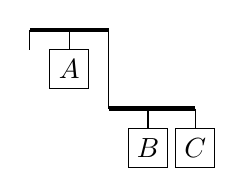
\begin{tikzpicture}
    \draw[ultra thick]
        (-4,2)--(-3,2)
        (-3,1)--(-1.9,1)
    ;
    \draw
        (-4,2)--(-4,1.75)
        (-3.5,2)--(-3.5,1.75)
        (-3.75,1.25) rectangle (-3.25,1.75)
        node[anchor=center]at(-3.5,1.5){$\bm{A}$}
        (-3,1)--(-3,2)
        (-2.5,1)--(-2.5,.75)
        (-2.25,.25)rectangle(-2.75,.75)
        node[anchor=center]at(-2.5,.5){$\bm{B}$}
        (-1.9,1)--(-1.9,.75)
        (-2.15,.25)rectangle(-1.65,.75)
        node[anchor=center]at(-1.9,.5){$\bm{C}$}
    ;
\end{tikzpicture}
}}
    =
    \vcenter{\hbox{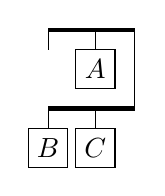
\begin{tikzpicture}
    \draw[ultra thick]
        (-.1,2)--(1,2)
        (-.1,1)--(1,1)
    ;
    \draw
        (1,1)--(1,2)
        (-.1,2)--(-.1,1.75)
        (.5,2)--(.5,1.75)
        (.25,1.25)rectangle(.75,1.75)
        node[anchor=center]at(.5,1.5){$\bm{A}$}
        (-.1,1)--(-.1,.75)
        (-.35,.25)rectangle(.15,.75)
        node[anchor=center]at(-.1,.5){$\bm{B}$}
        (.5,1)--(.5,.75)
        (.25,.25)rectangle(.75,.75)
        node[anchor=center]at(.5,.5){$\bm{C}$}
    ;
\end{tikzpicture}
}}
    =
    \vcenter{\hbox{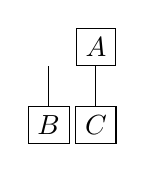
\begin{tikzpicture}
    \draw
        node[anchor=south, draw, rectangle](A1)at(3.65,1.25){$\bm{A}$}
        node[anchor=north, draw, rectangle](B1)at(3.05,.75){$\bm{B}$}
        node[anchor=north, draw, rectangle](C1)at(3.65,.75){$\bm{C}$}
        (A1.south)--(C1.north)
        (B1.north)-- ++(0,.5)
    ;
\end{tikzpicture}
}}
    -
    \vcenter{\hbox{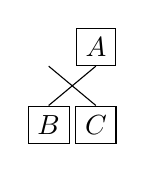
\begin{tikzpicture}
    \draw
        node[anchor=south, draw, rectangle](A2)at(5.4,1.25){$\bm{A}$}
        node[anchor=north, draw, rectangle](B2)at(4.8,.75){$\bm{B}$}
        node[anchor=north, draw, rectangle](C2)at(5.4,.75){$\bm{C}$}
        (A2.south)--(B2.north)
        (C2.north)--++(-.6,.5)
    ;
\end{tikzpicture}
}}
\end{equation*}


\subsubsection{ベクトル四重積}

\begin{equation*}
    (\bm{A}\times\bm{B})\cdot(\bm{C}\times\bm{D})
    =
    \det\mqty(
        \bm{A}\cdot\bm{C}
        &
        \bm{B}\cdot\bm{C}
        \\
        \bm{A}\cdot\bm{D}
        &
        \bm{B}\cdot\bm{D}
    )
\end{equation*}
行列式を使って表すことが多い.
行列式による表式が見やすいわけではないが, Levi-Civita記号の縮約公式が
\begin{align*}
    \epsilon_{ijm}\epsilon_{klm}
    =
    \det\mqty(
        \delta_{ik} & \delta_{il}
        \\
        \delta_{jk} & \delta_{jl}
    )
\end{align*}
と表されることを考慮すると自明であろう.
\begin{equation*}
    \vcenter{\hbox{\begin{tikzpicture}
    \coordinate(origin)at(0,2);
    \draw[ultra thick]
        (origin)--++(1.1,0)
        ($(origin)-(0,1)$)--++(1.1,0)
    ;
    \draw
        (origin)--++(0,-1)
        ++(.5,0)--++(0,-.25)
        node[anchor=north,draw,rectangle](C1){$\bm{C}$}
        ++(.6,.25)--++(0,-.25)
        node[anchor=north,draw,rectangle](D1){$\bm{D}$}
        ++(0,1.25)--++(0,-.25)
        node[anchor=north,draw,rectangle](B1){$\bm{B}$}
        ++(-.6,.25)--++(0,-.25)
        node[anchor=north,draw,rectangle](A1){$\bm{A}$}
    ;
\end{tikzpicture}
}}
    =
    \vcenter{\hbox{\begin{tikzpicture}
    \coordinate(origin)at(3,2);
    \draw
        ($(origin)+(0,-.25)$)
        node[anchor=north,draw,rectangle](A2){$\bm{A}$}
        ++(.6,0)
        node[anchor=north,draw,rectangle](B2){$\bm{B}$}
        ++(-.6,-1)
        node[anchor=north,draw,rectangle](C2){$\bm{C}$}
        ++(.6,0)
        node[anchor=north,draw,rectangle](D2){$\bm{D}$}
        (A2.south)--(C2.north)
        (B2.south)--(D2.north)
    ;
\end{tikzpicture}
}}
    -
    \vcenter{\hbox{\input{img/vector/A-DB-C.tex}}}
\end{equation*}



\subsection{スカラー・ベクトルの微分作用素}

Penroseのグラフ記法で扱う微分演算子は$\nabla$(ナブラ)である.
微分対象を円で囲い, 円から脚を伸ばすことで表現する.
これもまた図形的に表すことが可能である.
\begin{equation*}
    \nabla
    =
    \vcenter{\hbox{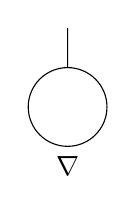
\begin{tikzpicture}
    \draw
    circle[radius=0.5]
    ++(0,.5)--++(0,.5)
    ++(0,-1.5)node[anchor=north]{$\nabla$}
    ;
\end{tikzpicture}
}}
\end{equation*}


\subsubsection{勾配 $\gradop$}

スカラーを円で囲って脚を伸ばす.
\begin{equation*}
    \gradop{f}=\nabla f
    =
    \vcenter{\hbox{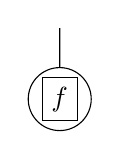
\begin{tikzpicture}
    \draw
    node[anchor=center,draw,rectangle]{$f$}
    circle[radius=0.4]
    ++(0,.4)--++(0,.5)
    ;
\end{tikzpicture}
}}
\end{equation*}


\subsubsection{発散 $\diver$}

ベクトルの脚と微分演算子の脚をつなげる.
\begin{equation*}
    \diver\bm{v}=\nabla\cdot\bm{v}
    =
    \vcenter{\hbox{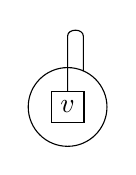
\begin{tikzpicture}
    \draw
    node[anchor=center,draw,rectangle](v){$\bm{v}$}
    (v.north)--++(0,.7)
    .. controls ++(0,.1) and ++(0,.1) .. ++(.2,0)
    --++(0,-.45)
    (v.center)circle[radius=.5]
    ;
\end{tikzpicture}
}}
\end{equation*}
脚はKroneckerの$\delta$を表すので$\partial_i\delta_{ij}v_j$を意味する.


\subsubsection{回転 $\rotop$}
\label{sec: rot}

単純な外積と表示は大きく変わらない.
ただし微分対象は演算子のすぐ右の脚に配置する.
\footnote{この追加ルールについては\ref{sec: div uv}を参照. }
\begin{equation*}
    \rotop\bm{v}=\nabla\times\bm{v}
    =
    \vcenter{\hbox{\begin{tikzpicture}
    \coordinate(origin)at(0,0);
    \draw
    (origin)--++(1,0)
    ++(0,-.05)--++(-1,0)
    (origin)--++(0,-.25)
    ++(.5,.25)--++(0,-.25)
    ($(origin)+(1,0)$)--++(0,-.25)
    node[anchor=north, draw, rectangle](v){$\bm{v}$}
    (v.center)circle[radius=.3]
    ($(origin)+(.5,-.25)$)--++(.2,-.2)
    ;
\end{tikzpicture}
}}
\end{equation*}


\subsubsection{ラプラシアン $\lapl$}
\label{sec: lapl}

2つの微分演算子の脚をつなぎ合わせる.
微分対象はスカラー・ベクトルを問わない.
\begin{equation*}
    \lapl f=\laplacian f
    =
    \vcenter{\hbox{\input{img/vector/lapl-f.tex}}},
    \qquad
    \lapl \bm{v}
    =
    \laplacian\bm{v}
    =
    \vcenter{\hbox{\begin{tikzpicture}
    \coordinate(origin2)at(2,0);
    \draw
        (origin2) node[anchor=center, draw, rectangle](v){$\bm{v}$}
        (v.north)--++(0,.5)
        ($(v.north)+(.2,.15)$)--++(0,.7)
        .. controls ++(0,.1) and ++(0,.1) .. ++(.2,0)
        --++(0,-.6)
        (v.center) circle[radius=.4]
        (v.center) circle[radius=.6]
    ;
\end{tikzpicture}
}}
\end{equation*}
$\partial_i\delta_{ij}\partial_jA$を表す.
特に微分対象がスカラーの場合, 直ちに$\diver\gradop f=\lapl f$が得られる.


\subsubsection{積の微分(Leibnitz rule)}

\begin{equation*}
    \nabla(AB)=\nabla(A)B+A\nabla(B)
\end{equation*}
微分作用素はLeibnitz ruleに従って展開可能である.
\begin{equation*}
    \vcenter{\hbox{\begin{tikzpicture}
    \coordinate(O1)at(0,0);
    \coordinate(O2)at(2.8,0);
    \coordinate(O3)at(5.6,0);
    \node[anchor=center]at(1.4,0){$=$};
    \node[anchor=center]at(4.2,0){$+$};
    \draw
    ($(O1)+(-.4,0)$) node[anchor=center,draw,rectangle]{$A$}
    ($(O1)+(.4,0)$) node[anchor=center,draw,rectangle]{$B$}
    (O1)circle[x radius=1,y radius=.4]
    ++(0,.4)--++(0,.5)
    ;
    \draw
    ($(O2)+(-.4,0)$) node[anchor=center,draw,rectangle](A){$A$}
    ($(O2)+(.4,0)$) node[anchor=center,draw,rectangle]{$B$}
    (A)circle[radius=.4]
    ++(0,.4)--++(0,.5)
    ;
    \draw
    ($(O3)+(-.4,0)$) node[anchor=center,draw,rectangle]{$A$}
    ($(O3)+(.4,0)$) node[anchor=center,draw,rectangle](B){$B$}
    (B)circle[radius=.4]
    ++(0,.4)--++(0,.5)
    ;
\end{tikzpicture}
}}
\end{equation*}


\subsubsection{微分順序交換}

$C^2$級関数(2階導関数が連続な関数)では微分順序の交換が可能である.
グラフ記法では円の内外を入れ替えることにほかならない.
\begin{equation*}
    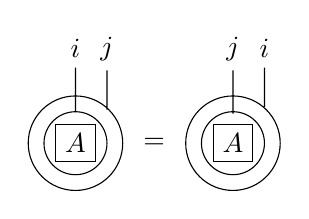
\begin{tikzpicture}
    \coordinate(origin1)at(0,0);
    \coordinate(origin2)at(2,0);
    \node at(0,1.2)[anchor=center](i1){$i$};
    \node at(.4,1.2)[anchor=center](j1){$j$};
    \node at(2.4,1.2)[anchor=center](i2){$i$};
    \node at(2.,1.2)[anchor=center](j2){$j$};
    \draw
    (origin1) node[anchor=center, draw, rectangle](A1){$A$}
    (i1.south)--++(0,-.55)
    (j1.south)--++(0,-.5)
    (A1.center) circle[radius=.4]
    (A1.center) circle[radius=.6]
    ;
    \draw
    (origin2) node[anchor=center, draw, rectangle](A2){$A$}
    (i2.south)--++(0,-.5)
    (j2.south)--++(0,-.55)
    (A2.center) circle[radius=.4]
    (A2.center) circle[radius=.6]
    ;
    \node[anchor=center]at(1,0){$=$};
\end{tikzpicture}

\end{equation*}
以降, 特に断りのない限り全ての量は$C^2$級であるとする.



\subsection{ベクトルの微分作用素にまつわる公式}

本節の公式は以下に示す5つの変形\textbf{のみ}を用いて導出が可能である.
\begin{itemize}
    \item Levi-Civita記号の反対称性(奇置換)
    \item Levi-Civita記号での偶置換
    \item Levi-Civita記号の縮約公式
    \item Leibnitz rule
    \item 微分順序交換
\end{itemize}
全ての導出はEinsteinの縮約記法を用いた方法と全く同じ手順である.


\subsubsection{$\rotop\gradop=0$}
\label{sec: rot grad}

\begin{equation*}
    \rotop\gradop f=\nabla\times\nabla f=0
\end{equation*}
微分順序の交換と反対称性を用いる.
\begin{equation*}
    \begin{tikzpicture}
    \coordinate(origin1)at(0,0);
    \coordinate(origin2)at(3,0);
    \coordinate(origin3)at(6,0);
    \node at(1,-.5)[anchor=north, draw, rectangle](v1){$f$};
    \node at(4,-.5)[anchor=north, draw, rectangle](v2){$f$};
    \node at(7,-.5)[anchor=north, draw, rectangle](v3){$f$};
    \draw
    (origin1)--++(1,0)
    ++(0,-.05)--++(-1,0)
    (origin1)--++(0,-.25)
    ++(.5,.25)--++(0,-.25)
    ($(origin1)+(1,0)$)--++(0,-.4)
    (v1.center)circle[radius=.5]
    (v1.center)circle[radius=.4]
    ($(origin1)+(.5,-.25)$)--++(.15,-.15)
    ;
    \node at(2.25,-.5)[anchor=center]{$=$};
    \draw
    (origin2)--++(1,0)
    ++(0,-.05)--++(-1,0)
    (origin2)--++(0,-.25)
    ++(.5,.25)--++(0,-.25)
    ($(origin2)+(1,0)$)--++(0,-.3)
    (v2.center)circle[radius=.5]
    (v2.center)circle[radius=.4]
    ($(origin2)+(.5,-.25)$)--++(.25,-.25)
    ;
    \node at(5.25,-.5)[anchor=center]{$=-$};
    \draw
    (origin3)--++(1,0)
    ++(0,-.05)--++(-1,0)
    (origin3)--++(0,-.25)
    ++(.5,.25)--++(0,-.25)
    ($(origin3)+(1,0)$)--++(0,-.4)
    (v3.center)circle[radius=.5]
    (v3.center)circle[radius=.4]
    ($(origin3)+(.5,-.25)$)--++(.15,-.15)
    ;
\end{tikzpicture}

\end{equation*}
第1に微分順序交換, 第2に反対称.
左辺と右辺で$A=-A$の形になっているので値は$0$である.


\subsubsection{$\diver\rotop=0$}

\begin{equation*}
    \diver\rotop\bm{v}=\nabla\cdot(\nabla\times\bm{v})=0
\end{equation*}
\ref{sec: rot grad}と同様に示せる.
\begin{equation*}
    \begin{tikzpicture}
    \coordinate(origin1)at(0,0);
    \coordinate(origin2)at(3,0);
    \coordinate(origin3)at(6,0);
    \draw[ultra thick]
        (origin1)--++(1,0)
        (origin2)--++(1,0)
        (origin3)--++(1,0)
    ;
    \draw
        (origin1)--++(0,-.25)
        ++(.5,.25)--++(0,-.25)
        ($(origin1)+(1,0)$)--++(0,-.25)
        node[anchor=north, draw, rectangle](v1){$\bm{v}$}
        (v1.center)circle[radius=.3]
        (v1.center)circle[radius=.4]
        ($(origin1)+(0,-.25)$)--++(.6,-.3)
        ($(origin1)+(.5,-.25)$)--++(.2,-.2)
    ;
    \node at(2.25,-.5)[anchor=center]{$=$};
    \draw
        (origin2)--++(0,-.25)
        ++(.5,.25)--++(0,-.25)
        ($(origin2)+(1,0)$)--++(0,-.25)
        node[anchor=north, draw, rectangle](v2){$\bm{v}$}
        (v2.center)circle[radius=.3]
        (v2.center)circle[radius=.4]
        ($(origin2)+(0,-.25)$)--++(.7,-.3)
        ($(origin2)+(.5,-.25)$)--++(.1,-.1)
    ;
    \node at(5.25,-.5)[anchor=center]{$=-$};
    \draw
        (origin3)--++(0,-.25)
        ++(.5,.25)--++(0,-.25)
        ($(origin3)+(1,0)$)--++(0,-.25)
        node[anchor=north, draw, rectangle](v3){$\bm{v}$}
        (v3.center)circle[radius=.3]
        (v3.center)circle[radius=.4]
        ($(origin3)+(0,-.25)$)--++(.6,-.3)
        ($(origin3)+(.5,-.25)$)--++(.2,-.2)
    ;
\end{tikzpicture}

\end{equation*}
第1に微分順序交換, 第2に反対称.
やはり左辺と右辺で$A=-A$の形になっているので値は$0$となる.


\subsubsection{$\diver\gradop=\lapl$}

\begin{equation*}
    \diver\gradop f=\nabla\cdot\nabla f=\lapl f
\end{equation*}
\ref{sec: lapl}で紹介したが, 公式として再掲する.
\begin{equation*}
    \lapl f=\laplacian f
    =
    \vcenter{\hbox{\input{img/vector/lapl-f.tex}}}
\end{equation*}


\subsubsection{$\gradop(fg)=g\gradop f+f\gradop g$}

\begin{align*}
    &\gradop(fg)=(\gradop f)g+f(\gradop g)
    \\
    &\nabla(fg)=(\nabla f)g+f(\nabla g)
\end{align*}
Leibnitz ruleで展開する.
\begin{equation*}
    \begin{tikzpicture}
    \coordinate(origin1)at(0,0);
    \coordinate(origin2)at(2.8,0);
    \coordinate(origin3)at(5.6,0);
    \node[anchor=center]at(1.4,0){$=$};
    \node[anchor=center]at(4.2,0){$+$};
    \draw
    ($(origin1)+(-.4,0)$) node[anchor=center,draw,rectangle]{$f$}
    ($(origin1)+(.4,0)$) node[anchor=center,draw,rectangle]{$g$}
    (origin1)circle[x radius=1,y radius=.4]
    ++(0,.4)--++(0,.5)
    ;
    \draw
    ($(origin2)+(-.4,0)$) node[anchor=center,draw,rectangle](A){$f$}
    ($(origin2)+(.4,0)$) node[anchor=center,draw,rectangle]{$g$}
    (A)circle[radius=.4]
    ++(0,.4)--++(0,.5)
    ;
    \draw
    ($(origin3)+(-.4,0)$) node[anchor=center,draw,rectangle]{$f$}
    ($(origin3)+(.4,0)$) node[anchor=center,draw,rectangle](B){$g$}
    (B)circle[radius=.4]
    ++(0,.4)--++(0,.5)
    ;
\end{tikzpicture}

\end{equation*}
物理学においては, 数式でも然りだが, 誤解を生む形でなければベクトルのスカラー倍を表すのに必ずしもスカラー・ベクトルの順で配する必要はない.
グラフ記法でも同様である.


\subsubsection{$\diver(fv)=\gradop f\cdot v+f\diver v$}

\begin{align*}
    &\diver(f\bm{v})=\gradop f\cdot\bm{v}+f\diver\bm{v}
    \\
    &\nabla(f\bm{v})=\nabla f\cdot\bm{v}+f\nabla\cdot\bm{v}
\end{align*}
これもまたLeibnitz ruleで展開する.
\begin{equation*}
    \begin{tikzpicture}
    \coordinate(origin1)at(0,0);
    \coordinate(origin2)at(2.8,0);
    \coordinate(origin3)at(5.6,0);
    \node[anchor=center]at(1.4,0){$=$};
    \node[anchor=center]at(4.2,0){$+$};
    \draw
    ($(origin1)+(-.4,0)$) node[anchor=center,draw,rectangle]{$f$}
    ($(origin1)+(.4,0)$) node[anchor=center,draw,rectangle](v1){$\bm{v}$}
    (v1.north)--++(0,.7)
    (origin1)circle[x radius=1,y radius=.4]
    ++(0,.4)--++(0,.5)
    .. controls ++(0,.2) and ++(0,.2) .. ++(.4,0)
    ;
    \draw
    ($(origin2)+(-.4,0)$) node[anchor=center,draw,rectangle](f2){$f$}
    ($(origin2)+(.4,0)$) node[anchor=center,draw,rectangle](v2){$\bm{v}$}
    (f2)circle[radius=.4]
    (v2.west)--++(-.155,0)
    ;
    \draw
    ($(origin3)+(-.4,0)$) node[anchor=center,draw,rectangle]{$f$}
    ($(origin3)+(.4,0)$) node[anchor=center,draw,rectangle](v3){$\bm{v}$}
    (v3)circle[radius=.4]
    ++(.2,.35)--++(0,.5)
    (v3.north)--++(0,.65)
    .. controls ++(0,.1) and ++(0,.1) .. ++(.2,0)
    ;
\end{tikzpicture}

\end{equation*}


\subsubsection{$\diver(u\times v)=\rotop u\cdot v-u\cdot\rotop v$}
\label{sec: div uv}

\begin{align*}
    &\diver(\bm{u}\times\bm{v})=\rotop\bm{u}\cdot\bm{v}-\bm{u}\cdot\rotop\bm{v}
    \\
    &\nabla\cdot(\bm{u}\times\bm{v})=(\nabla\times\bm{u})\bm{v}-\bm{u}\cdot(\nabla\times\bm{v})
\end{align*}
Leibnitz ruleに加えて反対称性を用いる.
\begin{equation*}
    \begin{tikzpicture}
    \coordinate(origin1)at(0,0);
    \coordinate(origin2)at(3,0);
    \coordinate(origin3)at(6,0);
    \coordinate(origin4)at(3,-1.5);
    \coordinate(origin5)at(6,-1.5);
    \draw[ultra thick]
        (origin1)--++(1,0)
        (origin2)--++(1.5,0)
        (origin3)--++(1.5,0)
        (origin4)--++(1.5,0)
        (origin5)--++(1.5,0)
    ;
    \draw
        (origin1)--++(0,-.25)
        ++(.5,.25)--++(0,-.25)
        node[anchor=north, draw, rectangle](u1){$\bm{u}$}
        ($(origin1)+(1,0)$)--++(0,-.25)
        node[anchor=north, draw, rectangle](v1){$\bm{v}$}
        ($(u1.center)!.5!(v1.center)$)circle[x radius=.7, y radius=.3]
        ($(origin1)+(0,-.25)$)--++(.1,-.1)
    ;
    \node at(2.125,-.5)[anchor=center]{$=$};
    \draw
        (origin2)--++(0,-.25)
        ++(.75,.25)--++(0,-.25)
        node[anchor=north, draw, rectangle](u2){$\bm{u}$}
        ($(origin2)+(1.5,0)$)--++(0,-.25)
        node[anchor=north, draw, rectangle](v2){$\bm{v}$}
        (u2.center)circle[radius=.3]
        ($(origin2)+(0,-.25)$)--++(.45,-.3)
    ;
    \node at(5.25,-.5)[anchor=center]{$+$};
    \draw
        (origin3)--++(0,-.25)
        ++(.75,.25)--++(0,-.25)
        node[anchor=north, draw, rectangle](u3){$\bm{u}$}
        ($(origin3)+(1.5,0)$)--++(0,-.25)
        node[anchor=north, draw, rectangle](v3){$\bm{v}$}
        (v3.center)circle[radius=.3]
        ($(origin3)+(0,-.25)$)|-++(1.4,-.5)
    ;
    \node at(2.125,-2)[anchor=center]{$=$};
    \draw
        (origin4)--++(0,-.25)
        ++(.75,.25)--++(0,-.25)
        node[anchor=north, draw, rectangle](u4){$\bm{u}$}
        ($(origin4)+(1.5,0)$)--++(0,-.25)
        node[anchor=north, draw, rectangle](v4){$\bm{v}$}
        (u4.center)circle[radius=.3]
        ($(origin4)+(0,-.25)$)--++(.45,-.3)
    ;
    \node at(5.25,-2)[anchor=center]{$-$};
    \draw
        (origin5)--++(0,-.25)
        node[anchor=north, draw, rectangle](u5){$\bm{u}$}
        ++(.75,.25)--++(0,-.25)
        ($(origin5)+(1.5,0)$)--++(0,-.25)
        node[anchor=north, draw, rectangle](v5){$\bm{v}$}
        (v5.center)circle[radius=.3]
        ($(origin5)+(.75,-.25)$)|-++(.45,-.2)
    ;
\end{tikzpicture}

\end{equation*}
\ref{sec: rot}で示した「rotにおいて微分対象は微分作用素のすぐ右の脚につなげる」ルールに従うようにする.


\subsubsection{$\rotop(fv)=\gradop f\times v+f\rotop v$}

\begin{align*}
    &\rotop(f\bm{v})=\gradop f\times\bm{v}+f\:\rotop\bm{v}
    \\
    &\nabla\times(f\bm{v})=\nabla f\times\bm{v}+f\nabla\times\bm{v}
\end{align*}
Leibnitz ruleによる展開.
\begin{equation*}
    \begin{tikzpicture}
    \coordinate(origin1)at(0,0);
    \coordinate(origin2)at(3,0);
    \coordinate(origin3)at(6,0);
    \draw[ultra thick]
    (origin1)--++(1.5,0)
    (origin2)--++(1.5,0)
    (origin3)--++(1.5,0)
    ;
    \draw
        (origin1)--++(0,-.25)
        ++(1.5,.25)--++(0,-.4)
        node[anchor=north, draw, rectangle](v1){$\bm{v}$}
        ++(-.5,.075) node[anchor=north, draw, rectangle](f1){$f$}
        (v1.west)circle[x radius=.7, y radius=.5]
        ($(origin1)+(.6,0)$)--++(0,-.45)
    ;
    \node at(2.5,-.5)[anchor=center]{$=$};
    \draw
        (origin2)--++(0,-.25)
        ++(1.5,.25)--++(0,-.4)
        node[anchor=north, draw, rectangle](v2){$\bm{v}$}
        ($(origin2)+(.6,0)$)--++(0,-.25)
        ++(0,-.5) node[anchor=center,draw,rectangle](f2){$f$}
        (f2.center)circle[radius=.5]
    ;
    \node at(5.25,-.5)[anchor=center]{$+$};
    \draw
        (origin3)--++(0,-.25)
        ++(1.5,.25)--++(0,-.4)
        node[anchor=north, draw, rectangle](v3){$\bm{v}$}
        ($(origin3)+(.5,0)$)--++(0,-.25)
        |-++(.5,-.2)
        ($(origin3)+(-.1,-.8)$) node[anchor=center,draw,rectangle](f3){$f$}
        (v3.center)circle[radius=.5]
    ;
\end{tikzpicture}

\end{equation*}
微分の内外を遵守する限り$f$の位置は問わない.


\subsubsection{$\rotop(u\times v)=(v\cdot\gradop)u+u\diver v-v\diver u-(u\cdot\gradop)v$}

\begin{align*}
    &\rotop(\bm{u}\times\bm{v})
    =
    (\bm{v}\cdot\gradop)\bm{u}
    +
    \bm{u}\:\diver\bm{v}
    -
    \bm{v}\:\diver\bm{u}
    -
    (\bm{u}\cdot\gradop)\bm{v}
    \\
    &\nabla\times(\bm{u}\times\bm{v})
    =
    (\bm{v}\cdot\nabla)\bm{u}
    +
    \bm{u}(\nabla\cdot\bm{v})
    -
    \bm{v}(\nabla\cdot\bm{u})
    -
    (\bm{u}\cdot\nabla)\bm{v}
\end{align*}
Levi-Civita記号の縮約公式とLeibnitz ruleによって導出.
\begin{equation*}
    \begin{tikzpicture}
    \coordinate(origin1)at(0,0);
    \node at(1.8,-1)[anchor=center]{$=$};
    \coordinate(origin2)at(2.75,-.5);
    \node at(4.1,-1)[anchor=center]{$-$};
    \coordinate(origin3)at(5,-.5);
    \node at(1.8,-2.75)[anchor=center]{$=$};
    \coordinate(origin4)at(2.75,-2);
    \node at(4.3,-2.75)[anchor=center]{$+$};
    \coordinate(origin5)at(5,-2);
    \node at(6.6,-2.75)[anchor=center]{$-$};
    \coordinate(origin6)at(7.5,-2);
    \node at(8.9,-2.75)[anchor=center]{$-$};
    \coordinate(origin7)at(9.5,-2);
    % LHS
    \draw [ultra thick]
        (origin1)--++(1.1,0)
        ($(origin1)-(0,1.)$)--++(1.1,0)
    ;
    \draw
        (origin1)--++(0,-.25)
        ++(.6,.25)--++(0,-.25) node[anchor=north](dv1){}
        ++(.5,.25)--++(0,-1.0)
        ($(origin1)-(0,1.)$)--++(0,-.25) node[anchor=north,draw,rectangle](u1){$\bm{u}$}
        ++(.6,.25)--++(0,-.25) node[anchor=north,draw,rectangle](v1){$\bm{v}$}
        ($(u1.center)!.5!(v1.center)$)circle[x radius=.7,y radius=.5]
        (dv1.north)--++(-.3,-.7)
    ;
    % RHS up
    \draw
        (origin2)--++(0,-.5)
        node[anchor=north,draw,rectangle](u2){$\bm{u}$}
        node at ++(.6,0)[anchor=north,draw,rectangle](v2){$\bm{v}$}
        (v2.north)--++(0,.5)
        .. controls ++(0,.2) and ++(0,.2) .. ++(-.2,0)
        -- ++(0,-.2)
        ($(u2.center)!.5!(v2.center)$) circle[x radius=.7,y radius=.5]
    ;
    \draw
        (origin3)--++(.6,-.5)
        node[anchor=north,draw,rectangle](v3){$\bm{v}$}
        node at ++(-.6,0)[anchor=north,draw,rectangle](u3){$\bm{u}$}
        (u3.north)--++(.6,.5)
        .. controls ++(.1,.1) and ++(0,.1) .. ++(.2,0)
        -- ++(0,-.35)
        ($(u3.center)!.5!(v3.center)$) circle[x radius=.7,y radius=.5]
    ;
    % RHS down
    \draw
        (origin4)--++(0,-.5)
        node[anchor=north,draw,rectangle](u4){$\bm{u}$}
        ++(.8,0) node[anchor=north,draw,rectangle](v4){$\bm{v}$}
        (u4)circle[radius=.4]
        (v4.west)--++(-.155,0)
    ;
    \draw
        (origin5)--++(0,-.5)
        node[anchor=north,draw,rectangle](u5){$\bm{u}$}
        ++(.8,0) node[anchor=north,draw,rectangle](v5){$\bm{v}$}
        (v5)circle[radius=.4]
        (v5.north)--++(0,.5)
        .. controls ++(0,.1) and ++(0,.1) .. ++(.2,0)
        --++(0,-.35)
    ;
    \draw
        (origin6)--++(0,-.5)
        node[anchor=north,draw,rectangle](u6){$\bm{u}$}
        ++(.8,0) node[anchor=north,draw,rectangle](v6){$\bm{v}$}
        (u6.center)circle[radius=.4]
        (v6.north)--++(0,.5)
        (origin6) .. controls ++(0,.1) and ++(0,.1) .. ++(.2,0)
        --++(0,-.35)
    ;
    \draw
        ($(origin7)+(0,-.5)$) node[anchor=north,draw,rectangle](u7){$\bm{u}$}
        ++(.8,0) node[anchor=north,draw,rectangle](v7){$\bm{v}$}
        (v7.north)--++(0,.5)
        (v7.center)circle[radius=.4]
        (u7.east)--++(.155,0)
    ;
\end{tikzpicture}

\end{equation*}


\subsubsection{$\rotop\rotop=\gradop\diver-\lapl$}

\begin{align*}
    &\rotop\rotop\bm{v}=\gradop\diver\bm{v}-\lapl\bm{v}
    \\
    &\nabla\times(\nabla\times\bm{v})=\nabla(\nabla\cdot\bm{v})-(\nabla\cdot\nabla)\bm{v}
\end{align*}
Levi-Civita記号の縮約公式と微分順序交換から.
\begin{equation*}
    \begin{tikzpicture}
    \coordinate(origin1)at(0,0);
    \node at(1.8,-1)[anchor=center]{$=$};
    \coordinate(origin2)at(2.75,-.5);
    \node at(3.6,-1)[anchor=center]{$-$};
    \coordinate(origin3)at(4.5,-.5);
    \node at(5.4,-1)[anchor=center]{$=$};
    \coordinate(origin4)at(6.25,-.5);
    \node at(7.1,-1)[anchor=center]{$-$};
    \coordinate(origin5)at(8,-.5);
    % LHS
    \draw
    (origin1)--++(1.1,0)
    ++(0,-.05)--++(-1.1,0)
    ++(0,.05)--++(0,-.25)
    ++(.6,.25)--++(0,-.25) node[anchor=north](dv1){}
    ++(.5,.25)--++(0,-1.05)
    --++(-1.1,0)
    ++(0,.05)--++(1.1,0)
    ++(-.5,0)--++(0,-.25) node[anchor=north,draw,rectangle](v1){$\bm{v}$}
    (v1.center)circle[radius=.3]
    (v1.center)circle[radius=.4]
    (dv1.north)--++(.2,-.85)
    ($(origin1)+(0,-1)$)|-++(.3,-.4)
    ;
    % RHS up
    \draw
    (origin2)--++(0,-.5)
    node[anchor=north,draw,rectangle](v2){$\bm{v}$}
    (v2.north)--++(0,.5)
    .. controls ++(0,.1) and ++(0,.1) .. ++(-.2,0)
    -- ++(0,-.35)
    (v2.center)circle[radius=.4]
    (v2.center)circle[radius=.3]
    ($(v2.center)+(.15,.25)$)--++(0,.45)
    ;
    \draw
    (origin3)--++(0,-.5)
    node[anchor=north,draw,rectangle](v3){$\bm{v}$}
    (v3.north)--++(0,.5)
    ($(v3.north)+(.1,.2)$)--++(0,.4)
    .. controls ++(0,.1) and ++(0,.1) .. ++(.2,0)
    --++(0,-.7)
    (v3.center) circle[radius=.4]
    (v3.center) circle[radius=.3]
    ;
    \draw
    (origin4)--++(0,-.5)
    node[anchor=north,draw,rectangle](v4){$\bm{v}$}
    (v4.north)--++(0,.5)
    .. controls ++(0,.1) and ++(0,.1) .. ++(-.1,0)
    -- ++(0,-.425)
    (v4.center)circle[radius=.4]
    (v4.center)circle[radius=.3]
    ($(v4.center)+(.15,.375)$)--++(0,.45)
    ;
    \draw
    (origin5)--++(0,-.5)
    node[anchor=north,draw,rectangle](v5){$\bm{v}$}
    (v5.north)--++(0,.5)
    ($(v5.north)+(.1,.2)$)--++(0,.4)
    .. controls ++(0,.1) and ++(0,.1) .. ++(.2,0)
    --++(0,-.7)
    (v5.center) circle[radius=.4]
    (v5.center) circle[radius=.3]
    ;
\end{tikzpicture}

\end{equation*}


\subsubsection{$\gradop(u\cdot v)=v\times\rotop u+(v\cdot\gradop)u+u\times\rotop v+(u\cdot\gradop)v$}

\begin{align*}
    &
    \gradop(\bm{u}\cdot\bm{v})
    =
    \bm{v}\times\rotop\bm{u}+(\bm{v}\cdot\gradop)\bm{u}
    +
    \bm{u}\times\rotop\bm{v}+(\bm{u}\cdot\gradop)\bm{v}
    \\
    &
    \nabla(\bm{u}\cdot\bm{v})
    =
    \bm{v}\times(\nabla\times\bm{u})+(\bm{v}\cdot\nabla)\bm{u}
    +
    \bm{u}\times(\nabla\times\bm{v})+(\bm{u}\cdot\nabla)\bm{v}
\end{align*}
初手は順当にLeibnitz ruleで展開する.
\begin{equation}
    \label{figeq: vector: grad-uv1}
    \vcenter{\hbox{\begin{tikzpicture}
    \coordinate(origin1)at(0,0);
    \coordinate(origin2)at(2.8,0);
    \coordinate(origin3)at(5.6,0);
    \node[anchor=center]at(1.4,0){$=$};
    \node[anchor=center]at(4.2,0){$+$};
    \draw
    ($(origin1)+(-.4,0)$) node[anchor=center,draw,rectangle](u1){$\bm{u}$}
    ($(origin1)+(.4,0)$) node[anchor=center,draw,rectangle](v1){$\bm{v}$}
    (origin1)circle[x radius=1,y radius=.4]
    ++(0,.4)--++(0,.5)
    (u1.east)--(v1.west)
    ;
    \draw
    ($(origin2)+(-.4,0)$) node[anchor=center,draw,rectangle](u2){$\bm{u}$}
    ($(origin2)+(.4,0)$) node[anchor=center,draw,rectangle](v2){$\bm{v}$}
    (u2)circle[radius=.4]
    ++(0,.4)--++(0,.5)
    (u2.east)--(v2.west)
    ;
    \draw
    ($(origin3)+(-.4,0)$) node[anchor=center,draw,rectangle](u3){$\bm{u}$}
    ($(origin3)+(.4,0)$) node[anchor=center,draw,rectangle](v3){$\bm{v}$}
    (v3)circle[radius=.4]
    ++(0,.4)--++(0,.5)
    (u3.east)--(v3.west)
    ;
\end{tikzpicture}
}}
\end{equation}
展開した形に相当する演算がないので, 各項Levi-Civita記号の縮約公式から得られたものとみて計算する.
右辺第1項は次のLevi-Civita記号の縮約公式から現れる.
\begin{equation*}
    \begin{tikzpicture}
    \coordinate(origin1)at(0,0);
    \node at(1.8,-1)[anchor=center]{$=$};
    \coordinate(origin2)at(3,-1);
    \node at(4.1,-1)[anchor=center]{$-$};
    \coordinate(origin3)at(5,-.25);
    % LHS
    \draw[ultra thick]
        (origin1)--++(1.1,0)
        ($(origin1)-(0,1)$)--++(1.1,0)
    ;
    \draw
        (origin1)--++(0,-.25)
        ++(.6,.25)--++(0,-.25) node[anchor=north,draw,rectangle](v1){$\bm{v}$}
        ++(.5,.25)--++(0,-1.)
        ($(origin1)-(0,1)$)--++(0,-.25) node[anchor=north](dv1){}
        ++(.6,.25)--++(0,-.25) node[anchor=north,draw,rectangle](u1){$\bm{u}$}
        (u1.center)circle[radius=.3]
        (dv1.north)|-++(.3,-.3)
    ;
    % RHS up
    \draw
        ($(origin2)+(-.4,0)$) node[anchor=center,draw,rectangle](u2){$\bm{u}$}
        ($(origin2)+(.4,0)$) node[anchor=center,draw,rectangle](v2){$\bm{v}$}
        (u2)circle[radius=.4]
        ++(0,.4)--++(0,.5)
        (u2.east)--(v2.west)
    ;
    \draw
        (origin3)--++(0,-.5)
        node[anchor=north,draw,rectangle](u3){$\bm{u}$}
        ++(.8,0) node[anchor=north,draw,rectangle](v3){$\bm{v}$}
        (u3)circle[radius=.4]
        (v3.west)--++(-.155,0)
    ;
\end{tikzpicture}

\end{equation*}
この右辺第2項を移項したものが\eqref{figeq: vector: grad-uv1}第1項に一致する.
\eqref{figeq: vector: grad-uv1}第2項は$\bm{u},\bm{v}$を入れ替えたものに他ならない.
結局以下の図式を得る.
\begin{equation*}
    \begin{tikzpicture}
    \coordinate(origin1)at(0,0);
    \coordinate(origin2)at(2.5,1);
    \coordinate(origin3)at(5,.5);
    \coordinate(origin4)at(7.5,1);
    \coordinate(origin5)at(10,.5);
    \node[anchor=center]at(1.75,0){$=$};
    \node[anchor=center]at(4.2,0){$+$};
    \node[anchor=center]at(6.75,0){$+$};
    \node[anchor=center]at(9.2,0){$+$};

    % LHS
    \draw
        ($(origin1)+(-.4,0)$) node[anchor=center,draw,rectangle](u1){$\bm{u}$}
        ($(origin1)+(.4,0)$) node[anchor=center,draw,rectangle](v1){$\bm{v}$}
        (origin1)circle[x radius=1,y radius=.4]
        ++(0,.4)--++(0,.5)
        (u1.east)--(v1.west)
    ;
    % 1st
    \draw[ultra thick]
        (origin2)--++(1.1,0)
        ($(origin2)-(0,1)$)--++(1.1,0)
    ;
    \draw
        (origin2)--++(0,-.25)
        ++(.6,.25)--++(0,-.25) node[anchor=north,draw,rectangle](v1){$\bm{v}$}
        ++(.5,.25)--++(0,-1.0)
        ($(origin2)-(0,1)$)--++(0,-.25) node[anchor=north](dv1){}
        ++(.6,.25)--++(0,-.25) node[anchor=north,draw,rectangle](u1){$\bm{u}$}
        (u1.center)circle[radius=.3]
        (dv1.north)|-++(.3,-.3)
    ;
    % 2nd
    \draw
        (origin3)--++(0,-.5)
        node[anchor=north,draw,rectangle](u3){$\bm{u}$}
        ++(.8,0) node[anchor=north,draw,rectangle](v3){$\bm{v}$}
        (u3)circle[radius=.4]
        (v3.west)--++(-.155,0)
    ;
    % 3rd
    \draw[ultra thick]
        (origin4)--++(1.1,0)
        ($(origin4)-(0,1)$)--++(1.1,0)
    ;
    \draw
        (origin4)--++(0,-.25)
        ++(.6,.25)--++(0,-.25) node[anchor=north,draw,rectangle](v1){$\bm{u}$}
        ++(.5,.25)--++(0,-1.0)
        ($(origin4)-(0,1)$)--++(0,-.25) node[anchor=north](dv1){}
        ++(.6,.25)--++(0,-.25) node[anchor=north,draw,rectangle](u1){$\bm{v}$}
        (u1.center)circle[radius=.3]
        (dv1.north)|-++(.3,-.3)
    ;
    % 4th
    \draw
        (origin5)--++(0,-.5)
        node[anchor=north,draw,rectangle](u3){$\bm{v}$}
        ++(.8,0) node[anchor=north,draw,rectangle](v3){$\bm{u}$}
        (u3)circle[radius=.4]
        (v3.west)--++(-.155,0)
    ;
\end{tikzpicture}

\end{equation*}


\subsubsection{$\lapl(fg)=(\lapl f)g+2\:\gradop f\cdot\gradop g+f(\lapl g)$}

\begin{align*}
    &\lapl(fg)
    =
    (\lapl f)g+2\:\gradop f\cdot\gradop g+f(\lapl g)
    \\
    &\nabla\cdot\nabla(fg)
    =
    (\nabla\cdot\nabla f)g+2(\nabla f)\cdot(\nabla g)+f(\nabla\cdot\nabla g)
\end{align*}
2回にわたってLeibnitz ruleを使う.
\begin{equation*}
    \begin{tikzpicture}
    \coordinate(origin1)at(0,0);
    \coordinate(origin2)at(2.8,0);
    \coordinate(origin3)at(5.6,0);
    \coordinate(origin4)at(2.8,-2);
    \coordinate(origin5)at(5.6,-2);
    \coordinate(origin6)at(8.4,-2);
    \coordinate(origin7)at(11.2,-2);
    \node[anchor=center]at(1.4,0){$=$};
    \node[anchor=center]at(4.2,0){$+$};
    \node[anchor=center]at(1.4,-2){$=$};
    \node[anchor=center]at(4.2,-2){$+$};
    \node[anchor=center]at(7,-2){$+$};
    \node[anchor=center]at(9.8,-2){$+$};
    % LHS
    \draw
    ($(origin1)+(-.4,0)$) node[anchor=center,draw,rectangle]{$f$}
    ($(origin1)+(.4,0)$) node[anchor=center,draw,rectangle]{$g$}
    (origin1)circle[x radius=1,y radius=.4]
    (origin1)circle[x radius=1.1,y radius=.5]
    ++(0,.4)--++(0,.5)
    .. controls ++(.1,.2) .. ++(.2,0)
    --++(0,-.4)
    ;
    % RHS up
    \draw
    ($(origin2)+(-.4,0)$) node[anchor=center,draw,rectangle](A){$f$}
    ($(origin2)+(.4,0)$) node[anchor=center,draw,rectangle]{$g$}
    (A)circle[radius=.4]
    ++(0,.4)--++(0,.5)
    (origin2)circle[x radius=1.1,y radius=.5]
    ++(0,.5)--++(0,.4)
    .. controls ++(0,.1) and ++(0,.1) .. ++(-.4,0)
    ;
    \draw
    ($(origin3)+(-.4,0)$) node[anchor=center,draw,rectangle]{$f$}
    ($(origin3)+(.4,0)$) node[anchor=center,draw,rectangle](B){$g$}
    (B)circle[radius=.4]
    ++(0,.4)--++(0,.5)
    (origin3)circle[x radius=1.1,y radius=.5]
    ++(0,.5)--++(0,.4)
    .. controls ++(0,.1) and ++(0,.1) .. ++(.4,0)
    ;
    % RHS down
    \draw
    ($(origin4)+(-.4,0)$) node[anchor=center,draw,rectangle](A){$f$}
    ($(origin4)+(.4,0)$) node[anchor=center,draw,rectangle]{$g$}
    (A)circle[radius=.4]
    ++(0,.4)--++(0,.5)
    .. controls ++(0,.1) and ++(0,.1) .. ++(.2,0)
    --++(0,-.45)
    (A)circle[radius=.5]
    ;
    \draw
    ($(origin5)+(-.5,0)$) node[anchor=center,draw,rectangle](A){$f$}
    ($(origin5)+(.5,0)$) node[anchor=center,draw,rectangle](B){$g$}
    (A)circle[radius=.4]
    ++(.4,0)--++(.2,0)
    (B)circle[radius=.4]
    ;
    \draw
    ($(origin6)+(-.5,0)$) node[anchor=center,draw,rectangle](A){$f$}
    ($(origin6)+(.5,0)$) node[anchor=center,draw,rectangle](B){$g$}
    (A)circle[radius=.4]
    ++(.4,0)--++(.2,0)
    (B)circle[radius=.4]
    ;
    \draw
    ($(origin7)+(-.4,0)$) node[anchor=center,draw,rectangle]{$f$}
    ($(origin7)+(.4,0)$) node[anchor=center,draw,rectangle](B){$g$}
    (B)circle[radius=.4]
    ++(0,.4)--++(0,.5)
    .. controls ++(0,.1) and ++(0,.1) .. ++(.2,0)
    --++(0,-.45)
    (B)circle[radius=.5]
    ;
\end{tikzpicture}

\end{equation*}



\subsection{位置ベクトルの微分にまつわる公式}

位置ベクトルを$\nabla$で微分する際は次の縮約が可能である.
\begin{equation*}
    \pdv{r_i}r_j\bm{e}_j=\delta_{ij}\bm{e}_j
\end{equation*}
これをPenroseのグラフ記法で表すと, $\bm{r}$とそれを囲う円が消えて両端がつながったように表される.
\begin{equation*}
    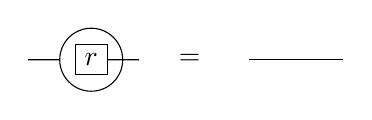
\begin{tikzpicture}
    \coordinate(origin1)at(0,0);
    \node at(1.25,0) [anchor=center]{$=$};
    \coordinate(origin2)at(2,0);
    \draw
    (origin1)node[anchor=center,draw,rectangle](r1){$\bm{r}$}
    (origin1.center)circle[radius=.4]
    ++(-.4,0)--++(-.4,0)
    (r1.east)--++(.4,0)
    ;
    \draw
    (origin2)--++(1.2,0)
    ;
\end{tikzpicture}

\end{equation*}
以下では「公式」とするにふさわしいものを拾っていくことにする.


\subsubsection{$\diver r=3$}

\begin{equation*}
    \diver\bm{r}=\nabla\cdot\bm{r}=\delta_{ii}=3
\end{equation*}
右辺の$3$は次元の数で, 4次元なら$4$, $n$次元なら$n$となる.
\begin{equation*}
    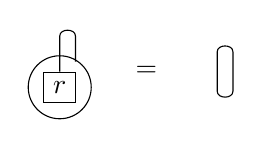
\begin{tikzpicture}
    \coordinate(origin1)at(0,0);
    \node at(1.1,0)[anchor=center]{$=$};
    \coordinate(origin2)at(2,-.25);
    \draw
    (origin1)node[anchor=north,draw,rectangle](r2){$\bm{r}$}
    (r2.center)circle[radius=.4]
    (r2.north)--++(0,.45)
    .. controls ++(0,.1) and ++(0,.1) .. ++(.2,0)
    --++(0,-.325)
    ;
    \draw
    (origin2)--++(0,.5)
    .. controls ++(0,.1) and ++(0,.1) ..++(.2,0)
    --++(0,-.5)
    .. controls ++(0,-.1) and ++(0,-.1) .. ++(-.2,0)
    ;
\end{tikzpicture}

\end{equation*}
右辺の環はKroneckerの$\delta$の両端がつながったものであり$\delta_{ii}$となる.
縮約のルールに則って3次元なら$i=1,2,3$で足し合わせる.


\subsubsection{$\rotop r=0$}

\begin{equation*}
    \rotop\bm{r}=\nabla\times\bm{r}=0
\end{equation*}
位置ベクトルの微分の縮約をとる.
\begin{equation*}
    \begin{tikzpicture}
    \coordinate(origin)at(0,0);
    \node at(2,0)[anchor=center]{$=$};
    \coordinate(origin2)at(3,0);
    \draw
    (origin)--++(1,0)
    ++(0,-.05)--++(-1,0)
    (origin)--++(0,-.25)
    ++(.5,.25)--++(0,-.25)
    ($(origin)+(1,0)$)--++(0,-.25)
    node[anchor=north, draw, rectangle](v){$\bm{r}$}
    (v.center)circle[radius=.3]
    ($(origin)+(.5,-.25)$)--++(.2,-.2)
    ;
    \draw
    (origin2)--++(1,0)
    ++(0,-.05)--++(-1,0)
    (origin)--++(0,-.25)
    ++(.5,.25)--++(0,-.25)
    ($(origin2)+(1,0)$)--++(0,-.25)
    --++(-.5,0)
    (origin2)--++(0,-.25)
    ++(.5,.25)--++(0,-.25)
    ;
\end{tikzpicture}

\end{equation*}
右辺は$\epsilon_{ijk}\delta_{jk}=\epsilon_{ijj}$を表すので$0$である.



\end{document}
}}
    ,\qquad
    v^j
    =
    \vcenter{\hbox{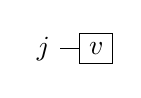
\begin{tikzpicture}
    \node at(0,0)[anchor=center, draw, rectangle](v){$v$};
    \draw
        (v.west)--++(-.25,0)node[left]{$j$}
    ;
\end{tikzpicture}
}}
    .
\end{equation*}

表記の都合上, 脚を上下から生やすことも少なくない.
その場合, 上の脚を行, 下の脚を列に対応させる.
\begin{equation*}
    A^i_j
    =
    \vcenter{\hbox{
        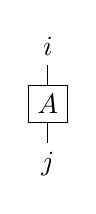
\begin{tikzpicture}
            \node at(0,0)[anchor=center, draw, rectangle](A){$A$};
            \draw
                (A.north)--++(0,.25)
                node[anchor=south]{$i$}
                (A.south)--++(0,-.25)
                node[anchor=north]{$j$}
            ;
        \end{tikzpicture}
    }}
\end{equation*}


\subsubsection{行列積}

行列積は脚をつなげて表される.
\begin{equation*}
    AB
    =
    \vcenter{\hbox{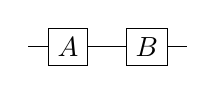
\begin{tikzpicture}
    \node at(0,0)[anchor=center, draw, rectangle](A){$A$};
    \node at(1,0)[anchor=center, draw, rectangle](B){$B$};
    \draw
        (A.west)--++(-.25,0)
        (A.east)--(B.west)
        (B.east)--++(.25,0)
    ;
\end{tikzpicture}
}}
\end{equation*}
実際, Kroneckerの$\delta$が\ref{sec: sec: Kronecker for tensor}で表されることを考慮すると, $(AB)^i_j=A^i_k\delta^k_lB^l_j=A^i_kB^k_j$になっている.

例えばベクトル$\bm{u},\bm{v}$と合わせて
\begin{equation*}
    \mqty(&\bm{u}&)
    \mqty(&&\\ &A&\\ &&)
    \mqty( {} \\ \bm{v} \\ {} )
    =
    u_iA^i_jv^j
    =
    \vcenter{\hbox{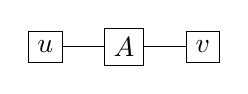
\begin{tikzpicture}
    \node at(0,0)[anchor=center, draw, rectangle](A){$A$};
    \node at(-1,0)[anchor=center, draw, rectangle](u){$\bm{u}$};
    \node at(1,0)[anchor=center, draw, rectangle](v){$\bm{v}$};
    \draw
        (u.east)--(A.west)
        (A.east)--(v.west)
    ;
\end{tikzpicture}
}}
\end{equation*}
とできる.
脚がないことから0階のテンソルすなわちスカラーであることが一目瞭然である.


\subsubsection{トレース}

トレースは行列から出た脚をつなげて表される.
\begin{equation*}
    \mathrm{tr}A
    =
    \vcenter{\hbox{\begin{tikzpicture}
    \coordinate(O)at(0,0);
    \draw
        (O)node[anchor=center, draw, rectangle](A){$A$}
        (A.west)--++(-.25,0)
        --++(0,.5)
        -|($(A.east)+(.25,0)$)
        --(A.east)
    ;
\end{tikzpicture}
}}
\end{equation*}
成分で見ると$A^i_j\delta^j_i=A_i^i$でたしかに対角和である.
脚がないのでスカラーである.


\subsubsection{転置}

行列の転置は脚の向きを反対側に捻じ曲げて表せる.
\begin{equation*}
    A^T
    =
    \vcenter{\hbox{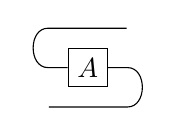
\begin{tikzpicture}
    \node at(0,0)[anchor=center, draw, rectangle](A){$A$};
    \draw
        (A.west)--++(-.25,0)
        .. controls ++(-.25,0) and ++(-.25,0) .. ++(0,.5)
        --++(1,0)
        (A.east)--++(.25,0)
        .. controls ++(.25,0) and ++(.25,0) .. ++(0,-.5)
        --++(-1,0)
    ;
\end{tikzpicture}
}}
\end{equation*}
転置を取っていることが自明な場合は転置前と同じダイアグラムにして省略することがある.


\subsubsection{和とスカラー倍}

行列の和とスカラー倍は文字式同様すれば良い.
$a, b\in\mathbb{C}$に対して
\begin{equation*}
    aA+bB
    =
    a\vcenter{\hbox{
        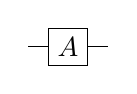
\begin{tikzpicture}
            \node at(0,0)[anchor=center, draw, rectangle](A){$A$};
            \draw(A.west)--++(-.25,0);
            \draw(A.east)--++(.25,0);
        \end{tikzpicture}
    }}
    +
    b
    \vcenter{\hbox{
        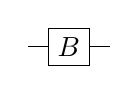
\begin{tikzpicture}
            \node at(0,0)[anchor=center, draw, rectangle](B){$B$};
            \draw(B.west)--++(-.25,0);
            \draw(B.east)--++(.25,0);
        \end{tikzpicture}
    }}
\end{equation*}
である.


\subsection{行列式と逆行列}
\label{sec: matrix: det and inverse}

形状が非自明なため説明が長くなる.
あらかじめ結論を示しておこう.
まず行列式は
\begin{equation}
    \label{eq: matrix: det M result}
    \det M
    =
    \frac{1}{n!}
    \vcenter{\hbox{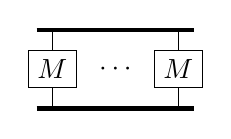
\begin{tikzpicture}
    \coordinate(O1)at(0,0);
    \coordinate(O2)at(0,-1);    
    \draw[ultra thick]
        (O1)--++(2,0)
        (O2)--++(2,0)
    ;
    \draw
        (O1)++(.2,0)--++(0,-.25)
        node[anchor=north, draw, rectangle](B1){$M$}
        (O2)++(.2,0)--(B1.south)
        (O1)++(1.8,0)--++(0,-.25)
        node[anchor=north, draw, rectangle](B2){$M$}
        (O2)++(1.8,0)--(B2.south)
        (O1)++(1,0)++(0,-.5)
        node[anchor=center]{$\cdots$}
    ;
\end{tikzpicture}
}}
\end{equation}
で表される.
余因子行列は
\begin{equation*}
    \tilde{M}
    =
    \frac{1}{(n-1)!}
    \vcenter{\hbox{\input{img/matrix/adjugate-nofactor.tex}}}
\end{equation*}
で, これによって逆行列は
\begin{equation*}
    M^{-1}
    =
    n
    \frac{\vcenter{\hbox{\input{img/matrix/adjugate-nofactor.tex}}}}{\vcenter{\hbox{\begin{tikzpicture}
    \coordinate(O1)at(0,0);
    \coordinate(O2)at(0,-1);    
    \draw[ultra thick]
        (O1)--++(2,0)
        (O2)--++(2,0)
    ;
    \draw
        (O1)++(.2,0)--++(0,-.25)
        node[anchor=north, draw, rectangle](B1){$M$}
        (O2)++(.2,0)--(B1.south)
        (O1)++(1.8,0)--++(0,-.25)
        node[anchor=north, draw, rectangle](B2){$M$}
        (O2)++(1.8,0)--(B2.south)
        (O1)++(1,0)++(0,-.5)
        node[anchor=center]{$\cdots$}
    ;
\end{tikzpicture}
}}}
\end{equation*}
とできる.


\subsubsection{行列式}
\label{sec: levicivita: determinant}

Penroseのグラフ記法で行列式を表そう.
$n\times n$行列の行列式は
\begin{align*}
    \det M
    =
    \sum_{\sigma\in\mathfrak{S}_n}
    \sgn(\sigma)M^1_{\sigma_1}\cdots M^n_{\sigma_n}
\end{align*}
で定義された.
ここに$\mathfrak{S}_n$は$n$次対称群(置換の集合)である.
置換の符号$\sgn(\sigma)$はLevi-Civita記号の正負に一致する.
すなわち$\sgn(\sigma)=\epsilon^{\sigma_1\cdots\sigma_n}_{1\cdots n}$
である.
縮約の際に添字が取りうる値を全て走ることに注意すると,
\begin{align*}
    \det M
    =
    \epsilon^{\sigma_1\cdots\sigma_n}_{1\cdots n}
    M^1_{\sigma_1}\cdots M^n_{\sigma_n}
\end{align*}
を得る.
Einsteinの縮約記法に従えば添字は一般に重複するが, Levi-Civita記号のため$\sigma_k$に重複がある項は0となる.
この形をそのままグラフ記法に落とし込むと行の添字を操作することが難しくなるので, 一見冗長だが
\begin{align}
    \label{eq: levicivita: det with levicivita}
    \det M
    =
    \frac{1}{n!}
    \epsilon^{\sigma_1\cdots\sigma_n}_{1\cdots n}
    \epsilon_{\tau_1\cdots\tau_n}^{1\cdots n}
    M^{\tau_1}_{\sigma_1}\cdots M^{\tau_n}_{\sigma_n}
\end{align}
とする.
先頭の係数は重複を割るために入れた.

これをグラフ記法で描くと以下のようになる.
\begin{equation}
    \label{eqfig: levicivita: determinant}
    \det M
    =
    \frac{1}{n!}
    \vcenter{\hbox{\begin{tikzpicture}
    \coordinate(O1)at(0,0);
    \coordinate(O2)at(0,-1);    
    \draw[ultra thick]
        (O1)--++(2,0)
        (O2)--++(2,0)
    ;
    \draw
        (O1)++(.2,0)--++(0,-.25)
        node[anchor=north, draw, rectangle](B1){$M$}
        (O2)++(.2,0)--(B1.south)
        (O1)++(1.8,0)--++(0,-.25)
        node[anchor=north, draw, rectangle](B2){$M$}
        (O2)++(1.8,0)--(B2.south)
        (O1)++(1,0)++(0,-.5)
        node[anchor=center]{$\cdots$}
    ;
\end{tikzpicture}
}}
\end{equation}


\subsubsection{余因子展開}

行列式が明示的に表せたので余因子展開も直感的に解釈できると期待される.
\begin{align}
    \label{eq: levicivita: cofactor expans in usual way}
    \det M
    =
    \sum_j (-1)^{i+j}M^i_j\det\mqty(
        M_1^1 & \cdots & M^1_{j-1} & M^1_{j+1} & \cdots & M^1_n
        \\
        \vdots & & \vdots & \vdots & & \vdots
        \\
        M^{i-1}_1 & \cdots & M^{i-1}_{j-1} & M^{i-1}_{j+1} & \cdots & M^{i-1}_n
        \\
        M^{i+1}_1 & \cdots & M^{i+1}_{j-1} & M^{i+1}_{j+1} & \cdots & M^{i+1}_n
        \\
        \vdots & & \vdots & \vdots & & \vdots
        \\
        M^n_1 & \cdots & M^n_{j-1} & M^n_{j+1} & \cdots & M_n^n
    )
\end{align}
ここで添字$i$は固定しているが, $i$も回した方が見通しが良い.
可能な添字の組み合わせ$(i,j)$全てで和をとると$i$の候補として$n$個の重複が現れるので, \eqref{eq: levicivita: det with levicivita}を利用して,
\begin{align*}
    \det M
    &=
    \frac{1}{n}
    \sum_{i,j} (-1)^{i+j}M^i_j
    \frac{1}{(n-1)!}
    \epsilon^{\sigma_1\cdots\sigma_{i-1}\sigma_{i+1}\cdots\sigma_n}_{1\cdots i-1,i+1\cdots n}
    \epsilon^{1\cdots j-1,j+1\cdots n}_{\tau_1\cdots\tau_{j-1}\tau_{j+1}\cdots\tau_n}
    M_{\sigma_1}^{\tau_1}\cdots M^{\tau_n}_{\sigma_n}
\end{align*}
である.
なお, $\sigma_k, \tau_k$はそれぞれ$\{1, \cdots, i-1, i+1, \cdots, n\}, \{1, \cdots, j-1, j+1, \cdots, n\}$すなわち$i$以外, $j$以外を走る.
% 符号$(-1)^{i+j}$もLevi-Civita記号の中に入れることができれば$n$階のLevi-Civita記号が現れ, \ref{eq: cofactor expansion in usual notation}に比べて遥かに簡単に構成できるようになる.
Levi-Civita記号部分が
\begin{align}
    \label{eq: levicivita: levicivita technique for cofactor expansion}
    \begin{split}
        \epsilon^{1\cdots i-1,i+1\cdots n}_{\sigma_1\cdots\sigma_{i-1}\sigma_{i+1}\cdots\sigma_n}
        \epsilon_{1\cdots j-1,j+1\cdots n}^{\tau_1\cdots\tau_{j-1}\tau_{j+1}\cdots\tau_n}
        &=
        \epsilon^{1\cdots i-1,i,i+1\cdots n}_{\sigma_1\cdots\sigma_{i-1},i,\sigma_{i+1}\cdots\sigma_n}
        \epsilon_{1\cdots j-1,j,j+1\cdots n}^{\tau_1\cdots\tau_{j-1},j,\tau_{j+1}\cdots\tau_n}
        \\
        &=
        \delta_i^{\sigma_i}\delta_{\tau_j}^j
        \epsilon^{1\cdots i-1,i,i+1\cdots n}_{\sigma_1\cdots\sigma_{i-1}\sigma_i\sigma_{i+1}\cdots\sigma_n}
        \epsilon_{1\cdots j-1,j,j+1\cdots n}^{\tau_1\cdots\tau_{j-1}\tau_j\tau_{j+1}\cdots\tau_n}
        \\
        &=
        (-1)^{i+j}
        \delta_i^{\sigma_i}\delta_{\tau_j}^j
        \epsilon^{1\cdots i-1,i,i+1\cdots n}_{\sigma_i\sigma_1\cdots\sigma_{i-1}\sigma_{i+1}\cdots\sigma_n}
        \epsilon_{1\cdots j-1,j,j+1\cdots n}^{\tau_j\tau_1\cdots\tau_{j-1}\tau_{j+1}\cdots\tau_n}
    \end{split}
\end{align}
となることに注意して,
\begin{align*}
    \det M
    &=
    \frac{1}{n}
    M^{\sigma_i}_{\tau_j}
    \frac{1}{(n-1)!}
    \epsilon^{1\cdots i-1,i,i+1\cdots n}_{\sigma_i\sigma_1\cdots\sigma_{i-1}\sigma_{i+1}\cdots\sigma_n}
    \epsilon_{1\cdots j-1,j,j+1\cdots n}^{\tau_j\tau_1\cdots\tau_{j-1}\tau_{j+1}\cdots\tau_n}
    M^{\sigma_1}_{\tau_1}\cdots M_{\tau_n}^{\sigma_n}
\end{align*}
である.

行列式の図式\eqref{eqfig: levicivita: determinant}と比べると, $M^{\sigma_i}_{\tau_j}$は先頭の記号$M$に対応し, 残りの$n-1$個が余因子とみなせる.
係数$1/(n-1)!$は余因子の重複を解消し, $1/n$は先頭の$M$の添字のうち片方について重複を解消している.
\begin{equation*}
    \begin{tikzpicture}
    \coordinate(O1)at(0,0);
    \coordinate(O2)at(0,-1);
    \node at(-.8,-.5)[anchor=east]{$\displaystyle\det M=\frac{1}{\dim M!}$};
    \draw[ultra thick]
        (O1)--++(3,0)
        (O2)--++(3,0)
    ;
    \draw
        (O1)++(.2,0)
        .. controls ++(0,-.25) and ++(0,.25) .. ($(O1)+(-.4,-.25)$)
        node[anchor=north, draw, rectangle](B0){$M$}
        (B0.south) .. controls ++(0,-.25) and ++(0,.25) .. ($(O2)+(.2,0)$)
        (O1)++(1.,0)--++(0,-.25)
        node[anchor=north, draw, rectangle](B1){$M$}
        (O2)++(1.,0)--(B1.south)
        (O1)++(2.6,0)--++(0,-.25)
        node[anchor=north, draw, rectangle](B2){$M$}
        (O2)++(2.6,0)--(B2.south)
        (O1)++(1.8,0)++(0,-.5)
        node[anchor=center]{$\cdots$}
    ;
\end{tikzpicture}

\end{equation*}
もし\eqref{eq: levicivita: cofactor expans in usual way}同様に片方の添字を回さないのであれば, 先頭の$M$の足が片方切れ, また重複を消す係数$1/n$が消える.
切れた足の添字は同一である.
\begin{equation*}
    \input{img/matrix/cofactor-expans-i.tex}
\end{equation*}
この状態は行列$M$と余因子行列$\tilde{M}$の行列積の$ii$成分になっているはずである.
したがって余因子行列は次の形で書けることがわかる.
\begin{equation}
    \label{eqfig: levicivita: adjugate mat}
    \tilde{M}
    =
    \frac{1}{(\dim M-1)!}
    \vcenter{\hbox{\input{img/matrix/adjugate-nofactor.tex}}}
\end{equation}

この表式を検証しよう.
一般に余因子行列の定義は数式で表すと煩雑になるのであった.
\begin{align*}
    \tilde{M}_i^j
    =
    (-1)^{i+j}
    \det\mqty(
        M_1^1 & \cdots & M_1^{i-1} & M_1^{i+1} & \cdots & M_1^n
        \\
        \vdots & \ddots & \vdots & & \ddots & \vdots
        \\
        M_{j-1}^1 & \cdots & M_{j-1}^{i-1} & M_{j-1}^{i+1} & \cdots & M_{j-1}^n
        \\
        M_{j+1}^1 & \cdots & M_{j+1}^{i-1} & M_{j+1}^{i+1} & \cdots & M_{j+1}^n
        \\
        \vdots & \ddots & \vdots & & \ddots & \vdots
        \\
        M_n^1 & \cdots & M_n^{i-1} & M_n^{i+1} & \cdots & M_n^n
    )
\end{align*}
一旦Levi-Civita記号を用いた表示にすると見通しが良い.
整理のため余因子行列の転置を考えると, \eqref{eq: levicivita: det with levicivita}にしたがって,
\begin{align*}
    \tilde{M}_j^i
    =
    \frac{(-1)^{i+j}}{(n-1)!}
    \epsilon_{1\cdots i-1,i+1\cdots n}^{\sigma_1\cdots\sigma_{i-1}\sigma_{i+1}\cdots\sigma_n}
    \epsilon^{1\cdots j-1,j+1\cdots n}_{\tau_1\cdots\tau_{j-1}\tau_{j+1}\cdots\tau_n}
    M_{\sigma_1}^{\tau_1}
    \cdots
    M_{\sigma_{i-1}}^{\tau_{i-1}}
    M_{\sigma_{i+1}}^{\tau_i}
    M_{\sigma_{i+2}}^{\tau_{i+1}}
    \cdots
    M_{\sigma_j}^{\tau_{j-1}}
    M_{\sigma_{j+1}}^{\tau_{j+1}}
    \cdots
    M_{\sigma_n}^{\tau_n}
\end{align*}
という形になる.
なお, $\sigma, \tau$はそれぞれ$\{1, \cdots, i-1, i+1, \cdots, n\}, \{1, \cdots, j-1, j+1, \cdots, n\}$を走る.
Levi-Civita記号部分が\eqref{eq: levicivita: levicivita technique for cofactor expansion}に一致することに注意して, 転置まで取れば
\begin{align*}
    \tilde{M}_i^j
    =
    \frac{1}{(n-1)!}
    \delta_{\sigma_i}^j\delta_i^{\tau_j}
    \epsilon_{1\cdots i-1,i,i+1\cdots n}^{\sigma_i\sigma_1\cdots\sigma_{i-1}\sigma_{i+1}\cdots\sigma_n}
    \epsilon^{1\cdots j-1,j,j+1\cdots n}_{\tau_j\tau_1\cdots\tau_{j-1}\tau_{j+1}\cdots\tau_n}
    M_{\sigma_1}^{\tau_1}
    \cdots
    M_{\sigma_{i-1}}^{\tau_{i-1}}
    M_{\sigma_{i+1}}^{\tau_i}
    \cdots
    M_{\sigma_j}^{\tau_{j-1}}
    M_{\sigma_{j+1}}^{\tau_{j+1}}
    \cdots
    M_{\sigma_n}^{\tau_n}
\end{align*}
である.

これほど大量の添字が並ぶと, なおのことグラフ記法の有用性がわかる.
各添字が走る領域を考慮すると, 図式は\eqref{eqfig: levicivita: adjugate mat}が対応する.
上の太線が$\tau_k$の置換に, 下の太線が$\sigma_k$の置換に当たる.
係数の$(n-1)!$は後ろの$n-1$個の成分の並べ替えに対応していることが一目でわかるだろう.


\subsubsection{逆行列}

余因子行列まで求まれば逆行列の計算も難しくない.
定義によれば正則行列$M$について, $M^{-1}=\tilde{M}/\det M$である.
したがって直ちに以下を得る.
\begin{equation}
    \label{eqfig: levicivita: inverse}
    M^{-1}
    =
    n
    \frac{\vcenter{\hbox{\input{img/matrix/adjugate-nofactor.tex}}}}{\vcenter{\hbox{\begin{tikzpicture}
    \coordinate(O1)at(0,0);
    \coordinate(O2)at(0,-1);    
    \draw[ultra thick]
        (O1)--++(2,0)
        (O2)--++(2,0)
    ;
    \draw
        (O1)++(.2,0)--++(0,-.25)
        node[anchor=north, draw, rectangle](B1){$M$}
        (O2)++(.2,0)--(B1.south)
        (O1)++(1.8,0)--++(0,-.25)
        node[anchor=north, draw, rectangle](B2){$M$}
        (O2)++(1.8,0)--(B2.south)
        (O1)++(1,0)++(0,-.5)
        node[anchor=center]{$\cdots$}
    ;
\end{tikzpicture}
}}}
\end{equation}

この空いている脚に$M$をつなぐと単位行列になることを確認しよう.
余因子行列に$M$をつないだ$M\tilde{M}$の成分は以下のようになる.
\begin{equation}
    \label{eqfig: levicivita: MMtilde}
    (M\tilde{M})^i_j
    =
    n
    \frac{\vcenter{\hbox{\input{img/matrix/cofactor-expans-ij.tex}}}}{\vcenter{\hbox{\begin{tikzpicture}
    \coordinate(O1)at(0,0);
    \coordinate(O2)at(0,-1);    
    \draw[ultra thick]
        (O1)--++(2,0)
        (O2)--++(2,0)
    ;
    \draw
        (O1)++(.2,0)--++(0,-.25)
        node[anchor=north, draw, rectangle](B1){$M$}
        (O2)++(.2,0)--(B1.south)
        (O1)++(1.8,0)--++(0,-.25)
        node[anchor=north, draw, rectangle](B2){$M$}
        (O2)++(1.8,0)--(B2.south)
        (O1)++(1,0)++(0,-.5)
        node[anchor=center]{$\cdots$}
    ;
\end{tikzpicture}
}}}
\end{equation}
これが単位行列であることを
\begin{enumerate}
    \item 対角行列である
    \item 対角成分が全て等しい
    \item 対角和が次元に等しい
\end{enumerate}
の手順で示していこう.

まずは\eqref{eqfig: levicivita: MMtilde}が対角行列であることを示す.
すなわち$i\neq j$で$(M\tilde{M})^i_j=0$となることを見れば良い.
添字を扱いやすくする目的で行成分に付け加えたLevi-Civita記号だが, ここでは外した方が見通しが良い.
Levi-Civita記号には各脚1本ずつに添字が割り当てられており, それぞれは異なって$1$から$n$まで全てをとりうる.
先頭は$j$で固定されているので, 先頭の$M$に加えて後ろ$n-1$本の中どれかにも$i$が入っている.
\begin{equation*}
    \vcenter{\hbox{\begin{tikzpicture}
    \draw
    node[anchor=south](i){$i$}
    (i.south)
    --++(0,-.2)
    .. controls ++(0,-.2) and ++(0,.2) .. ++(.3,-.5)
    --++(0,-.2)
    node[anchor=north]{$i$}
    ;
\end{tikzpicture}
}}
    \vcenter{\hbox{\begin{tikzpicture}
    \coordinate(O1)at(0,0);
    \coordinate(O2)at(0,-1);
    \draw[ultra thick]
        (O1)--++(3,0)
    ;
    \draw
        (O1)++(.2,0)
        --++(0,-.25)
        node[anchor=north, draw, rectangle](B0){$M$}
        (B0.south)--++(0,-.25)
        node[anchor=north]{$j$}
        (O1)++(1.8,0)--++(0,-.25)
        node[anchor=north, draw, rectangle](B1){$M$}
        (B1.south)--++(0,-.25)
        node[anchor=north]{$j$}
        (O1)++(2.6,-.5)
        node[anchor=center]{$\cdots$}
        (O1)++(1.,-.5)
        node[anchor=center]{$\cdots$}
    ;
\end{tikzpicture}
}}
    +(\mathrm{replacements})
\end{equation*}
この同じ添字$j$をぶら下げた$M$どうしを奇置換しても等価な形が現れるので, Levi-Civita記号にぶら下がる図式は値が$0$となる.
したがって$M\tilde{M}$は対角行列であることが示された.

今度は対角成分が等しい, すなわち$(M\tilde{M})_{ii}=(M\tilde{M})_{jj}$を示す.
\begin{equation*}
    (M\tilde{M})_{ii}
    \propto
    \pm
    \vcenter{\hbox{\begin{tikzpicture}
    \coordinate(O1)at(0,0);
    \coordinate(O2)at(0,-1);
    \draw[ultra thick]
        (O1)--++(2,0)
    ;
    \draw
        (O1)++(.2,0)
        --++(0,-.25)
        node[anchor=north, draw, rectangle](B0){$M$}
        (B0.south)--++(0,-.25)
        node[anchor=north]{$i$}
        (O1)++(1.8,0)--++(0,-.25)
        node[anchor=north, draw, rectangle](B1){$M$}
        (B1.south)--++(0,-.25)
        node[anchor=north]{$n$}
        (O1)++(1.,-.8)
        node[anchor=center]{$\cdots$}
        (O2)++(1.,-.5)
        % node[anchor=center]{$j$}
    ;
\end{tikzpicture}
}}
    +(\mathrm{replacements})
\end{equation*}
ただし符号は下付きの添字に対応する置換に合わせる.
どの並び順にしても, 下付き添字が$1$から$n$に順に並ぶよう置換を繰り返すと全て符号が$+$で揃うので, 値は成分によらない.

最後に\eqref{eqfig: levicivita: MMtilde}で脚をつなげると分母の$\det$から出た図式と一致するので, $\tr M\tilde{M}=n=\tr 1$である.

以上より$M\tilde{M}=1$である.
全く同様にして$\tilde{M}M=1$も示される.
$M$との行列積が単位行列となるので, \eqref{eqfig: levicivita: inverse}は逆行列に他ならない.


\subsection{行列式の性質}
\label{sec: matrix: properties of determinant}

ここまでに求めた行列式などのグラフ記法によって諸々の性質を証明していこう.

\subsubsection{定数倍の行列式}

\begin{equation*}
    \det(cA)=c^n\det A
\end{equation*}
Levi-Civita記号につながる$n$個全ての$A$が$c$倍される.
\begin{equation*}
    \vcenter{\hbox{
        \begin{tikzpicture}
            \draw[ultra thick](0,0)--++(2.7,0);
            \draw[ultra thick](0,-1)--++(2.7,0);
            \node at(.1,-.5)[anchor=center]{$c$};
            \node at(2,-.5)[anchor=center]{$c$};
            \draw
                (.6,0)--++(0,-.25)
                node[anchor=north,draw,rectangle](A1){$A$}
                (A1.south)--++(0,-.25)
                (2.5,0)--++(0,-.25)
                node[anchor=north,draw,rectangle](A2){$A$}
                (A2.south)--++(0,-.25)
            ;
            \node at(1.4,-.5)[anchor=center]{$\cdots$};
        \end{tikzpicture}
    }}
    =
    c^n
    \vcenter{\hbox{
        \begin{tikzpicture}
            \coordinate(O1)at(0,0);
            \coordinate(O2)at(0,-1);
            \draw[ultra thick]
                (O1)--++(2,0)
                (O2)--++(2,0)
            ;
            \draw
                (O1)++(.2,0)--++(0,-.25)
                node[anchor=north, draw, rectangle](B1){$A$}
                (O2)++(.2,0)--(B1.south)
                (O1)++(1.8,0)--++(0,-.25)
                node[anchor=north, draw, rectangle](B2){$A$}
                (O2)++(1.8,0)--(B2.south)
                (O1)++(1,0)++(0,-.5)
                node[anchor=center]{$\cdots$}
            ;
        \end{tikzpicture}
    }}
\end{equation*}


\subsubsection{行列積の行列式}

\begin{equation*}
    \det(AB)=\det(A)\det(B)
\end{equation*}

この導出に先立って, 添え字が$1$から$n$の値を取るようなLevi-Civita記号に$n$次元正方行列$A$が$n$個繋がったときに成り立つ公式
\begin{equation}
    \label{eq: matrix: insert Levi-Civita}
    \vcenter{\hbox{
        \begin{tikzpicture}
            \draw[ultra thick](0,0)--++(2,0);
            \draw
                (.2,0)--++(0,-.25)node[anchor=north, draw, rectangle](A){$A$}
                (A.south)--++(0,-.25)
                (1.75,0)--++(0,-.25)node[anchor=north, draw, rectangle](B){$A$}
                (B.south)--++(0,-.25)
            ;
            \node at(1,-.5)[anchor=center]{$\cdots$};
        \end{tikzpicture}
    }}
    =
    \frac{1}{n!}
    \vcenter{\hbox{
        \begin{tikzpicture}
            \draw[ultra thick]
                (0,0)--++(2,0)
                (0,-1)--++(2,0)
            ;
            \draw
                (.2,0)--++(0,-.25)node[anchor=north, draw, rectangle](A){$A$}
                (A.south)--++(0,-.5)
                (1.75,0)--++(0,-.25)node[anchor=north, draw, rectangle](B){$A$}
                (B.south)--++(0,-.5)
            ;
            \node at(1,-.5)[anchor=center]{$\cdots$};
            \node at(1,-1.3)[anchor=center]{$\cdots$};
        \end{tikzpicture}
    }}
    =
    \frac{1}{n!}
    \vcenter{\hbox{
        \begin{tikzpicture}
            \draw[ultra thick]
                (0,0)--++(2,0)
                (0,-1)--++(2,0)
                (0,-1.2)--++(2,0)
            ;
            \draw
                (.2,0)--++(0,-.25)node[anchor=north, draw, rectangle](A){$A$}
                (A.south)--++(0,-.25)
                (1.75,0)--++(0,-.25)node[anchor=north, draw, rectangle](B){$A$}
                (B.south)--++(0,-.25)
                (.2,-1.2)--++(0,-.5)
                (1.75,-1.2)--++(0,-.5)
            ;
            \node at(1,-.5)[anchor=center]{$\cdots$};
            \node at(1,-1.5)[anchor=center]{$\cdots$};
        \end{tikzpicture}
    }}
\end{equation}
を示す.
第二の等号は\eqref{eq: Levi-Civita: product of Levi-Civita}による.
左辺はそれぞれの$A$の交換について完全反対称なのでLevi-Civita記号に比例する.
あとは脚が$12\dots n$の順に並んでいるとき値が合致していることを確認すれば良い.
便宜上縮約をとる各線に全単射の置換$\sigma,\tau: \{1,\dots,n\}\to\{1,\dots,n\}$によってインデックスを振ると, 右辺は
\begin{equation*}
    \begin{split}
        \frac{1}{n!}
        \vcenter{\hbox{
            \begin{tikzpicture}
                \draw[ultra thick]
                    (0,0)--++(2,0)
                    (0,-1.5)--++(2,0)
                ;
                \draw
                    (.2,0)--++(0,-.5)node[anchor=north, draw, rectangle](A){$A$}
                    (A.south)--++(0,-1)node[anchor=north]{$1$}
                    (1.75,0)--++(0,-.5)node[anchor=north, draw, rectangle](B){$A$}
                    (B.south)--++(0,-1)node[anchor=north]{$n$}
                ;
                \node at(1,-.75)[anchor=center]{$\cdots$};
                \node at(.2,-.25)[anchor=west]{$\sigma(1)$};
                \node at(1.75,-.25)[anchor=west]{$\sigma(n)$};
                \node at(.2,-1.25)[anchor=west]{$\tau(1)$};
                \node at(1.75,-1.25)[anchor=west]{$\tau(n)$};
            \end{tikzpicture}
        }}
        &=
        \frac{1}{n!}
        \vcenter{\hbox{
            \begin{tikzpicture}
                \draw[ultra thick]
                    (0,0)--++(2,0)
                    (0,-1.5)--++(2,0)
                ;
                \draw
                    (.2,0)--++(0,-.5)node[anchor=north, draw, rectangle](A){$A$}
                    (A.south)--++(0,-1)node[anchor=north]{$1$}
                    (1.75,0)--++(0,-.5)node[anchor=north, draw, rectangle](B){$A$}
                    (B.south)--++(0,-1)node[anchor=north]{$n$}
                ;
                \node at(1,-.75)[anchor=center]{$\cdots$};
                \node at(.2,-.25)[anchor=east]{$\tau^{-1}(\sigma(1))$};
                \node at(1.75,-.25)[anchor=west]{$\tau^{-1}(\sigma(n))$};
                \node at(.2,-1.25)[anchor=east]{$1$};
                \node at(1.75,-1.25)[anchor=west]{$n$};
            \end{tikzpicture}
        }}
        \\
        &=
        \frac{\epsilon^{1\dots n}_{1\dots n}}{n!}
        \vcenter{\hbox{
            \begin{tikzpicture}
                \draw[ultra thick](0,0)--++(2,0);
                \draw
                    (.2,0)--++(0,-.5)node[anchor=north, draw, rectangle](A){$A$}
                    (A.south)--++(0,-.25)node[anchor=north]{$1$}
                    (1.75,0)--++(0,-.5)node[anchor=north, draw, rectangle](B){$A$}
                    (B.south)--++(0,-.25)node[anchor=north]{$n$}
                ;
                \node at(1,-.5)[anchor=center]{$\cdots$};
                \node at(.2,-.25)[anchor=east]{$\tau^{-1}(\sigma(1))$};
                \node at(1.75,-.25)[anchor=west]{$\tau^{-1}(\sigma(n))$};
            \end{tikzpicture}
        }}
    \end{split}
\end{equation*}
である.
縮約の総和は$\tau, \sigma$が任意の置換をとることに対応する.
$\{1,\dots,n\}\to\{1,\dots,n\}$の置換は総じて$n!$個存在する.
総和すると$\sigma,\tau$それぞれが$n!$通りの置換を走って$\tau^{-1}\circ\sigma$は$(n!)^2$通りの作り方ができる.
しかし$\tau^{-1}\circ\sigma$もまた置換であるため, 異なるものは$n!$しかない.
つまり
\begin{equation*}
    \sum_{\sigma\in\mathfrak{S}_n}
    \sum_{\tau\in\mathfrak{S}_n}
    \tau^{-1}\circ\sigma
    =
    n!\sum_{\sigma\in\mathfrak{S_n}}\sigma
\end{equation*}
なので, \eqref{eq: matrix: insert Levi-Civita}が成立する.

\eqref{eq: matrix: insert Levi-Civita}を使えば積の行列式は半ば自明に導出できる.
$n$次元正方行列$A, B$の積の行列式は
\begin{equation*}
    \det(AB)
    =
    \vcenter{\hbox{
        \begin{tikzpicture}
            \draw[ultra thick](0,0)--(2,0);
            \draw[ultra thick](0,-1.75)--(2,-1.75);
            \draw
                (.2,0)--++(0,-.25)
                node[anchor=north, draw, rectangle](A1){$A$}
                (A1.south)--++(0,-.25)
                node[anchor=north, draw, rectangle](B1){$B$}
                (B1.south)--++(0,-.25)
                (1.8,0)--++(0,-.25)
                node[anchor=north, draw, rectangle](A2){$A$}
                (A2.south)--++(0,-.25)
                node[anchor=north, draw, rectangle](B2){$B$}
                (B2.south)--++(0,-.25)
            ;
            \node at(1,-.8)[anchor=center]{$\cdots$};
        \end{tikzpicture}
    }}
    =
    \frac{1}{n!}
    \vcenter{\hbox{
        \begin{tikzpicture}
            \draw[ultra thick](0,0)--++(2,0);
            \draw[ultra thick](0,-1)--++(2,0);
            \draw[ultra thick](0,-1.2)--++(2,0);
            \draw[ultra thick](0,-2.2)--++(2,0);
            \draw
                (.2,0)--++(0,-.25)
                node[anchor=north,draw,rectangle](A1){$A$}
                (A1.south)--++(0,-.25)
                (1.8,0)--++(0,-.25)
                node[anchor=north,draw,rectangle](A2){$A$}
                (A2.south)--++(0,-.25)
            ;
            \draw
                (.2,-1.2)--++(0,-.25)
                node[anchor=north,draw,rectangle](B1){$B$}
                (B1.south)--++(0,-.25)
                (1.8,-1.2)--++(0,-.25)
                node[anchor=north,draw,rectangle](B2){$B$}
                (B2.south)--++(0,-.25)
            ;
            \node at(1,-.5)[anchor=center]{$\cdots$};
            \node at(1,-1.7)[anchor=center]{$\cdots$};
        \end{tikzpicture}
    }}
    =
    \det A\det B
\end{equation*}
なので, 積の行列式は行列式の積となる.


\subsubsection{逆行列の行列式}

\begin{equation*}
    \det(A^{-1})=1/\det(A)
\end{equation*}
$\det(AA^{-1})=\det A\det A^{-1}=1$から導出される.
特にグラフ記法を使う必要はない.
余因子行列の行列式が複雑なので, 上記の方法から導くのが圧倒的に簡単.


\subsubsection{余因子行列の行列式}

\begin{equation*}
    \det\tilde{A}
    =
    (\det A)^{n-1}
\end{equation*}
逆行列の定義と行列の定数倍の行列式から
\begin{equation*}
    \det A^{-1}
    =
    \det\qty(\frac{\tilde{A}}{\det A})
    =
    \frac{\det\tilde{A}}{(\det A)^n}
\end{equation*}
となることから導出可能.
これもグラフ記法は不要.


\subsubsection{転置行列の行列式}

\begin{equation*}
    \det A^T=\det A
\end{equation*}
脚が全て潰れたグラフは特別な向きを持たないので, $\det A$と区別がつかない.
\begin{equation*}
    \vcenter{\hbox{
        \begin{tikzpicture}
            \draw[ultra thick](0,0)--++(2,0);
            \draw[ultra thick](0,-1)--++(2,0);
            \node at(.5,-.5)[anchor=center, draw, rectangle](A){$A$};
            \draw
                (A.west)--++(-.1,0)
                ..controls++(-.5,0) and ++(0,-.1)..(.5,0)
                (A.east)--++(.1,0)
                ..controls++(.5,0)and++(0,.1)..(.5,-1)
            ;
            \node at(1.5,-.5)[anchor=center]{$\cdots$};
            \draw[<->, >=Stealth, dashed](2.1,-.05)arc(60:-60:.3 and .5);
        \end{tikzpicture}
    }}
    =
    \vcenter{\hbox{
        \begin{tikzpicture}
            \draw[ultra thick](0,0)--++(2,0);
            \draw[ultra thick](0,-1)--++(2,0);
            \node at(.5,-.5)[anchor=center, draw, rectangle](A){$A$};
            \draw
                (A.west)--++(-.1,0)
                ..controls++(-.5,0) and ++(0,.1)..(.5,-1)
                (A.east)--++(.1,0)
                ..controls++(.5,0)and++(0,-.1)..(.5,0)
            ;
            \node at(1.5,-.5)[anchor=center]{$\cdots$};
        \end{tikzpicture}
    }}
\end{equation*}



\end{document}
